\usepackage[utf8x]{inputenc}
\usepackage[german]{babel}
\usepackage{float}
\usepackage{multicol}
\usepackage{listings}
\usepackage{courier}
\lstset{inputencoding=utf8x, breaklines=true, basicstyle=\ttfamily\scriptsize}
\lstset{literate=%
{Ö}{{\"O}}1
{Ä}{{\"A}}1
{Ü}{{\"U}}1
{ß}{{\ss}}2
{ä}{{\"a}}1
{ö}{{\"o}}1
{ü}{{\"u}}1
}
\lstdefinelanguage{html}{
basicstyle=\ttfamily\scriptsize,
keywords={
  a,
  body,
  charset,
  div,
  font,
  h1,
  h2,
  head,
  href,
  html,
  id,
  img,
  link,
  media,
  meta,
  p,
  src,
  style,
  table,
  td,
  title,
  tr
}, 
keywordstyle=\color{black}\bfseries} 
\lstdefinelanguage{xml}{
basicstyle=\ttfamily\scriptsize,
keywords={
  creationdate,
  creator,
  edition,
  format,
  identifier,
  publisher,
  recordid,
  subject,
  title,
  type
}, 
keywordstyle=\color{black}\bfseries} 

\lstdefinelanguage{ruby}{basicstyle=\ttfamily\scriptsize}
%%%%%%%%%%%%%%%%%%%%%%%%%%%%%%%%%%%%%%%%%%%%%%%%%%%%%%%%%%%%%%%%%%%%%%%%%%%%%%%%%%%%%%
\title[Grundlagen: Informationstechnologie]{\beta Grundlagen: Informationstechnologie in Bibliotheken \beta}
\subtitle{\beta Dokument noch in Arbeit \beta}
\author{Sven Koesling}
\institute{ETH--Bibliothek}
\date{Herbst 2017}

%%%%%%%%%%%%%%%%%%%%%%%%%%%%%%%%%%%%%%%%%%%%%%%%%%%%%%%%%%%%%%%%%%%%%%%%%%%%%%%%%%%%%%

%%%%%%%%%%%%%%%%%%%%%%%%%%%%%%%%%%%%%%%%%%%%%%%%%%%%%%%%%%%%%%%%%%%%%%%%%%%%%%%%%%%%%%
% \includeonly{ 20151204 20151211 }
%%%%%%%%%%%%%%%%%%%%%%%%%%%%%%%%%%%%%%%%%%%%%%%%%%%%%%%%%%%%%%%%%%%%%%%%%%%%%%%%%%%%%%
\begin{document}

\begin{frame}
  \maketitle
\end{frame}

\only<article>{\tableofcontents}

\section{Einleitung: Von Nullen und Einsen}
\only<article>{
  Um die Konzepte hinter aktuellen Entwicklungen wie z.B. ,,Cloud'' und BigData verstehen zu können, benötigen wir ein wenig Grundlagenwissen. Das werden wir im Laufe der Lektionen aufbauen. Mit diesem Wissen wird uns dann die Logik hinter den Entwicklungen verständlich. 

  Dazu schauen wir zunächst auf die Geschichte des Internets, befassen uns mit der Technik und bauen Verständnis für die grundlegenden Konzepte auf. 

  Wir lernen verschiedene Möglichkeiten zur Speicherung von Daten kennen, werden die unterschiedlichen Typen von Datenbanken besprechen und feststellen, dass die Tabelle nicht immer die ideale Form für das Ablegen von Daten ist, geschweige denn für die Formatierung bzw. Darstellung.

  So kommen wir dann auf Grundlagen der Formatierung von Webinhalten, die Struktur von Webseiten und die Manipulation derselben durch Javascript, gehen auf Frameworks ein und kommen schliesslich auf Webapplikationen.

  Ein Exkurs zeigt uns, wie man die bisher erlernten Konzepte und Techniken zum automatisierten Testen von Webapplikationen nutzen kann, bevor wir dann klären, was die viel gerühmte ,,Cloud'' ist und wo wir in unserer Branche beim Thema BigData stehen.
}

\only<presentation>{
\begin{frame}[label=uebersicht]{Kursus / Übersicht}
  \begin{overprint}
    \onslide<1|handout:0>
      \textbf{01.12.2017 : Von Nullen und Einsen}
      \begin{itemize}
        \item Vorstellung und Überblick
        \item Die Entwicklung des Internets
        \item Server: Was ist das eigentlich?
      \end{itemize}
    
    \onslide<2|handout:0>
      \textbf{15.12.2017 : Internettechnologien I, Datenbanktechnologien I}
      \begin{itemize}
        \item IntT I: Dokumentformen, Skriptsprachen, Ajax, responsive Web
        \item DBT I: Datenbanktypen, Technologien, Einstieg SQL
      \end{itemize}
    
    \onslide<3|handout:0>
      \textbf{22.12.2017 : Internettechnologien II: von interaktiven Webseiten zu WebApps in der Cloud}
      \begin{itemize}
        \item das ,,DOM''
        \item Manipulation von Elementen mit JavaScript
        \item Der Einsatz von JavaScript Frameworks anhand von Primos neuem UI
        \item Exkurs: Einsatz der bisher gelernten Technologien zum automatisierten Testen von WebApplikationen
      \end{itemize}
    
    \onslide<4|handout:0>
      \textbf{19.01.2018 : Datenbanktechnologien II: BigData}
      \begin{itemize}
        \item kurze Wiederholung --- wo stehen wir?
        \item Klärung verschiedener Begriffe und Buzzwords
        \item Anwendungsszenarien, Anwendung in der ETH
        \item In Medias Res: BigData am Bsp. Logfiles, DataScience am Bsp. Benutzerdaten
      \end{itemize}
  \end{overprint}
\end{frame}
}

\only<article>{
  Zunächst wollen wir uns mit der Denkweise von Informatikern vertraut machen, die für ,,normale'' Menschen etwas gewöhnungsbedürftig sein kann. 

  Informatiker lachen beispielsweise herzlich über folgenden Satz:
}

\begin{frame}{\only<presentation>{Von Nullen und Einsen}}
  \begin{quote}
    Es gibt 10 Sorten von Menschen: Diejenigen, die das Binärsystem verstehen, und die Übrigen.\hfill (Autor unbekannt)
  \end{quote}
\end{frame}

\only<article>{
  Computer basieren darauf, dass man in Schaltkreisen den Strom an-- bzw. abschalten kann. Es gibt nur die zwei Zustände ,,AN'' und ,,AUS". Mathematisch ist das kein Problem, mit jeder Anzahl von Ziffern $>2$ lässt sich zählen. Aber die Wirklichkeit lässt sich nur näherungsweise damit beschreiben.

  Der Satz macht nur dann Spass, wenn man das Binärsystem kennt und versteht. Im täglichen Leben benutzen wir das Dezimalsystem. Zum besseren Verständnis nehmen wir an, dass jeder Zahl eine unendliche Anzahl von Stellen vorangestellt ist, die den Wert 0 haben. Also statt $1$ nehmen wir $00000001$ an (hier mit sieben Stellen vorneweg, weil sich eine unendliche Anzahl so schlecht aufschreiben lässt\ldots{}).

  Wir zählen die Ziffern von $0$ bis $9$ hoch, und wenn die Ziffern aufgebraucht sind, erhöhen wir die Stelle davor um eins und setzen die eben hochgezählte Ziffer auf $0$ zurück. So wird die Zahl $9$ ($00000009$), wenn man um eins erhöht, zu $10$ ($00000010$)

  \begin{center}
    \begin{tabular}{rrrrrrcl}
      0 & 0 & 0 & 0 & 0 & 0 & 0 & 9\tabularnewline
        &  &  &  &  &  & \multicolumn{1}{c|}{+1} & auf 0 zurücksetzen\tabularnewline
      0 & 0 & 0 & 0 & 0 & 0 & 1 & 0\tabularnewline
    \end{tabular}
  \end{center}

  Im Binärsystem stehen uns nur zwei Ziffern zur Verfügung. Aber zwei Ziffern reichen zum Zählen. Man wendet das gleiche Prinzip an. So wird die Zahl $1$ ($00000001$), wenn man um eins erhöht, zu $10$ ($00000010$). Jetzt ergibt der Witz einen Sinn. Der binäre Wert $10$ entspricht in unserem Dezimalsystem dem Wert zwei.
  }

\begin{frame}{Die Folge der ersten neun Binärzahlen\ldots{}}
  \begin{center}
    0, 1, 10, 11, 100, 101, 110, 111, 1000 \ldots{}
  \end{center}
\end{frame}
%
\begin{frame}{\ldots{}und die ,,Übersetzung"}
  \begin{center}
    \begin{tabular}{|r|c|}
      \hline 
      binär & dezimal\tabularnewline
      \hline 
      \hline 
      0 & 0\tabularnewline
      \hline 
      1 & 1\tabularnewline
      \hline 
      10 & 2\tabularnewline
      \hline 
      11 & 3\tabularnewline
      \hline 
      100 & 4\tabularnewline
      \hline 
      101 & 5\tabularnewline
      \hline 
      110 & 6\tabularnewline
      \hline 
      111 & 7\tabularnewline
      \hline 
    \end{tabular}
  \end{center}
\end{frame}

\only<article>{
  Leibniz schreibt Ende des 17. Jahrhunderts dazu: 
  \begin{quotation}
    \ldots{}deshalb ist der letzte Tag der vollkommenste und der Sabbat, denn an ihm ist alles geschaffen und erfüllt, und deshalb schreibt sich die 7 111, also ohne Null. Und nur wenn man die Zahlen bloß mit 0 und 1 schreibt, erkennt man die Vollkommenheit des siebenten Tages. \hfill (Gottfried Wilhelm Leibniz)
  \end{quotation}
  Ein Computer kann aktuell\footnote{Die zur Zeit in Entwicklung befindlichen Quantencomputer kennen auch noch ,,vielleicht". Aber obwohl erste Schritte vielversprechend sind, liegen Quantencomputer noch in weiter Ferne. Und Quantenphysiker denken noch schräger als Informatiker --- das möchte ich dem geneigten Leser nicht zumuten.} nur zwei Zustände darstellen: ,,AN'' und ,,AUS". Damit ist das Binärsystem für Computer zum Rechnen ideal.

  \begin{block}{Hinweis}
    Für uns wäre es aus verschiedenen Gründen sehr unpraktisch, im Binärsystem zu rechnen. Die Zahlen werden z.B. sehr schnell sehr lang. So braucht die Sieben im Binärsystem schon drei Stellen (111).
  \end{block}

  Zahlen können wir also genau umrechnen. Aber wie bilden beispielsweise Musik digital ab? 

  Man kann sich mit ,,AN'' / ,,AUS'' -- Zuständen einer Kurve annähern. Zunächst vereinfachen wir das Problem, indem wir statt Musik eine Sinuskurve zur Veranschaulichung benutzen. Das geht, weil ein Ton eine Summe von Schwingungen ist. Sinustöne sind sehr reine Töne, deren Schwingung sehr sauber der Sinuskurve entspricht.
  }
\begin{frame}{eine Sinuskurve}
  \begin{figure}
    \begin{center}  
      \includegraphics[width=0.8\textwidth]{pics/sinus-kurve}
    \end{center}
    \caption{Sinuskurve, Quelle: $\text{Computer:club}^2$, Urheber: Rolf Degen}
  \end{figure}
\end{frame}

\only<article>{
  Wir wollen mal versuchen, mit unseren zwei Zuständen eine solche Kurve zu erzeugen, indem wir sie auf Karos abbilden. Nehmen wir an, dass ein Karo dem Zustand ,,AN'' entspricht, kein Karo dem Zustand ,,AUS". Wenn man jetzt Karos zu einer Pyramide zusammenstellt und dahinter an der Basis genau so eine Pyramide nach unten zeigen lässt, erhält man eine Annäherung an eine Sinuskurve. Die Abbildung der Kurve sähe dann etwa aus wie folgt.
  }

\begin{frame}{eine grobe Annäherung}
  \begin{center}
    \includegraphics[width=0.8\textwidth]{pics/grobe-karos}
  \end{center}
\end{frame}

\only<article>{
  Je mehr Informationen bzw. ,,AN'' / ,,AUS'' -- Zustände wir nun verwenden, desto feiner wird die Annäherung an die Kurve:
  }

\begin{frame}{eine feinere Annäherung}
  \begin{center}
    \includegraphics[width=0.8\textwidth]{pics/feine-karos}
  \end{center}
\end{frame}

\only<article>{
  Wenn man mal von meinen mangelnden Zeichenkünsten absieht, kommt das Ganze der Kurve schon näher. Da unser Auge wie unser Ohr ein begrenzt feines Messinstrument ist, brauchen wir das Karo-- Muster nur klein genug zu machen (oder weit genug vom Augen zu entfernen) und können die Treppenstufen der Karos nicht mehr sehen bzw. das Unnatürliche im Ton nicht mehr hören.

  Mit ,,AN'' / ,,AUS'' -- Zuständen lässt sich also die Wirklichkeit näherungsweise beschreiben. 
  \begin{block}{Hinweis}
  Egal, wie leistungsfähig Computersysteme sind, oder noch sein werden, sie werden immer nur eine Annäherung bieten können.
  \end{block}
  Glücklicherweise ist unser Ohr als Messinstrument so unsensibel, dass wir die Näherungen nicht mehr vom Original unterscheiden können, solange sie nur fein genug sind. So konnte Ende der siebziger Jahre die Firma Philipps der digitalen Musikproduktion und --wiedergabe mit der Einführung des CD--Spielers kräftigen Schwung geben.

  Mit Bildern ist das Prinzip ähnlich: Je feiner die Treppen, je höher also die Informationsdichte, desto wirklichkeitsgetreuer wird das Bild wiedergegeben.
  }

\begin{frame}{}
  \begin{figure}
    \begin{center}  
      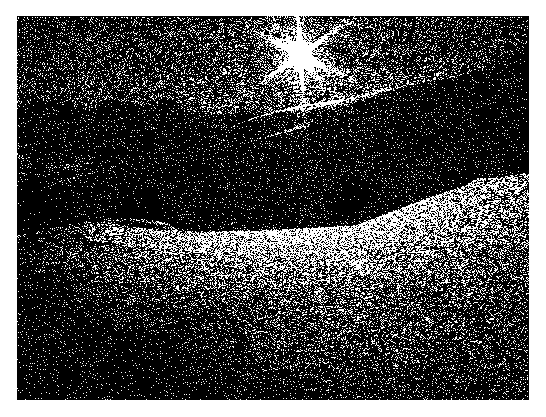
\includegraphics[width=0.8\textwidth]{pics/sw}
    \end{center}
    \caption{Ein Bild mit wenig Informationen (und kaum Speicherplatzbedarf: 123kb)}
  \end{figure}
\end{frame}
%
\begin{frame}{}
  \begin{figure}
    \begin{center}  
      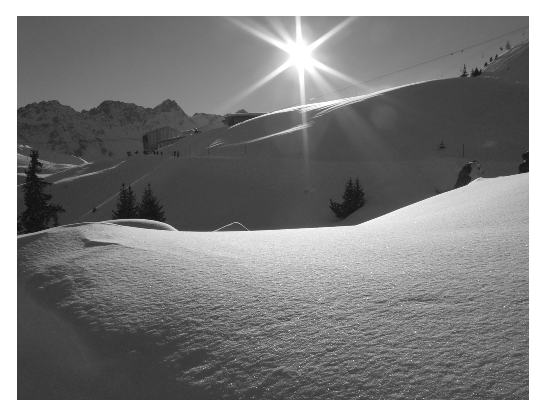
\includegraphics[width=0.8\textwidth]{pics/grau}
    \end{center}
    \caption{Ein Bild mit etwas mehr Informationen (und etwas mehr Speicherplatzbedarf:
551kb)}
  \end{figure}
\end{frame}
%
\begin{frame}{}
  \begin{figure}
    \begin{center}  
      \includegraphics[width=0.8\textwidth]{pics/farbe}
    \end{center}
    \caption{Ein Bild mit vielen Informationen (und noch mehr Speicherplatzbedarf:
1,1 MB)}
  \end{figure}
\end{frame}
%
\begin{frame}
\frametitle{Je mehr, desto besser}
  Je mehr ,,an'' / ,,aus'' Informationen wir einsetzen, desto näher ist das Ergebnis an der Wirklichkeit. Entsprechend steigen aber auch die benötigte Rechenleistung und der Speicherplatzbedarf an. 
\end{frame}
%
\only<article>{
  Das sind nun relativ kleine Beispielbilder gewesen. Rohbilder moderner Kameras benötigen aktuell 25 MB pro Bild, im semiprofessionellen Bereich das Doppelte, und im Mittelformat braucht es pro Bild ca. 600MB. Deshalb rechnet man mit speziellen Algorithmen ,,nicht benötigte'' Informationen aus den Daten heraus. Auch wenn der Leistungszuwachs von Computern aussergewöhnlich ist, stehen Speicher und Rechenpower nicht unbegrenzt zur Verfügung und sollten ganz normal als Ressource wahrgenommen werden, die man nicht verschwendet. 
  }

\subsection{Die Entwicklung des Internets}
%
\begin{frame}[<+->]{\only<presentation>{Die Entwicklung des Internets}}
\framesubtitle{Meilensteine}
  \begin{itemize}
    \item ARPA
    \item E-Mail
    \item www --- ein neuer Treiber
    \item Web Apps, Cloud Services und intelligente Kühlschränke
  \end{itemize}
\end{frame}

\subsubsection*{Der Vorläufer des Internets: Das Arpanet}
%%%%
%% Bis hier bin ich mit dem Refactoring gekommen
%%%%
\only<article>{
  Das Internet ist 1969 aus einer Zusammenarbeit des US--Verteidigungsministeriums und verschiedenen Forschungseinrichtungen entstanden. Obwohl sich das Gerücht hält, dass im kalten Krieg eine Technik aufgebaut werden sollte, die im Falle eines Atomschlages die Kommunikationsinfrastruktur erhalten kann, dürfte ein ausschlaggebender Grund für die Entwicklung die bessere Ausnutzung teurer Rechenkapazitäten gewesen sein. So entstand als Vorläufer des heutigen Internets das Arpanet. So oder so --- die Idee ist genial: Man teilt Kommunikation in kleine Päckchen auf und entwickelt Protokolle, die es ermöglichen, dass sich diese Päckchen ihren Weg selbständig vom Sender zum Empfänger suchen. Dabei gibt es nicht nur eine Leitung von A nach B, sondern ein fein verzweigtes Netzwerk mit unzähligen Knoten. Wenn nun eine Leitung blockiert ist, nimmt das Päckchen einfach einen anderen Weg. Übertragen wurden damals Übrigens noch keine Webseiten mit Bildern.
  }

\subsubsection{www : am CERN wird Internet--Geschichte geschrieben}

\only<article>{Das CERN spielt eine wichtige Rolle bei der Entwicklung des Internets, wie wir es heute kennen. Die Laboratorien des CERN liegen teilweise auf Schweizer Gebiet, teilweise auf französischem. Natürlich setzt jedes Land seine eigenen Computersysteme ein, was es damals unmöglich machte, Texte online auszutauschen. Mitte der achtziger Jahre nahm sich ein britischer Physiker und Informatiker namens Tim Berners--Lee dieses Problems an und entwickelt mit seinem Kollegen Robert Cailliau ein Konzept für ein weltweites Hypertext--Projekt, das sie 1990 veröffentlichen. Das daraus entstehende Protokoll ,,http" und die Auszeichnungssprache ,,html'' sind auch heute noch die Grundlagen des \textbf{W}orld \textbf{W}ide \textbf{W}eb. Dabei geht es darum Texte Über das Netzwerk zur Verfügung stellen zu können. Die Problematik, Texte universell für verschiedenste System darstellbar zu Übertragen, wird auch heute noch deutlich, wenn man z.B. eine Webseite auf einem Smartphone öffnet, die für den Desktop optimiert ist. Inzwischen sind die Texte um Bilder ,,bereichert", Filme werden Über das Internet gestreamt und Weltkarten in 3D betrachtet.
}

\subsubsection*{Das Internet der Dinge}

\only<article>{Da man nun immer mehr Leistung in immer kleinere Chips packen kann, können kleinste Dinge Funktionen bekommen, für die man früher ganze Rechenzentren benötigte. Wecker zeigen das Wetter an, Kalender berechnen die Wegzeit automatisch in Alarme mit ein, Navigationssysteme verwenden aktuelle und zu erwartende Verkehrsdaten, um die optimale Route zu bestimmen. Für all das benötigen die Dinge eine Verbindung zum Internet. Das wirft verschiedene Probleme auf: Sicherheit und Datenschutz sind ein Thema. Aber auch technisch braucht es neue Ansätze. So muss jeder, der an ihn gerichtete Informationen bekommen will, eindeutig identifizierbar sein. Die ursprünglich für diesen Zweck gemachte Adressierung (IPv4) hat für das Internet der Dinge viel zu wenig Adressen. Eine neue Technik zur Adressierung --- IPv6 --- ist vorhanden, setzt sich aber nur langsam durch.}

\begin{frame}
  \begin{figure}
    \begin{center}  
      \includegraphics[width=0.6\textwidth]{pics/internet}
    \end{center}
    \caption{Das Internet heute; Quelle: Wikipedia, Urheber: The Opte Project}
  \end{figure}
\end{frame}


\subsection{Server --- was ist das eigentlich?}
\begin{frame}[<+->]{\only<presentation>{Server --- was ist das eigentlich?}}
  \framesubtitle{die Themen:}
  \begin{itemize}
    \item Hardware
    \item Virtualisierung
    \item Software
  \end{itemize}
\end{frame}
%

\subsubsection*{Hardware}
\begin{frame}{}

\begin{figure}
\includegraphics[width=1\textwidth]{pics/MacMiniServer}

\caption{MacMini Server; Quelle: Gizmodo India}
\end{figure}

\end{frame}
\only<article>{
  Was ist ein Server? Im Grunde genommen ist jedes Gerät, das Dienstleistungen zur Verfügung stellt, ein Server. Wenn ich von meinem lokalen PC eine Webseite bereit stelle, die jemand anderes von seinem PC aufruft, ist mein PC in dem Moment ein Server.

  Ursprünglich war Rechenleistung so teuer, dass es in einer Institution nur einen riesigen Rechner in einem gut gekühlten Keller gab. Terminals ohne eigene Rechenkapazität stellten für eine Anzahl von Nutzern eine Verbindung zu diesem Rechner her, dessen Leistung unter allen Nutzern aufgeteilt wurde. Ende der 70er Jahre wurde die Technik so billig, dass mit dem Aufkommen der Personal Computers jeder seinen eigenen Rechner auf seinem Schreibtisch hatte. 

  Im Jahr 2000 wurden für den Aufbau einer Datenbank für kurze Texte noch 40.000 DM für einen Server der Firma SUN ausgegeben. Der Vorschlag, stattdessen einen Linux--PC für 5'000 DM einzusetzen war revolutionär\ldots{} und erfolgreich. Tatsächlich waren die PCs so leistungsfähig geworden, dass es keinen Grund mehr gab, das Achtfache zu investieren. 

  Woraus besteht nun ein PC?
}

\begin{frame}{die Komponenten eines PCs}

\begin{figure}
\includegraphics[width=1\textwidth]{pics/pc-komponenten}

\caption{die Komponenten eines PCs}
\end{figure}
\end{frame}

\only<article>{
  Das Herzstück des PCs ist der Prozessor --- der eigentliche Rechner. Damit Menschen mit ihm kommunizieren können, gibt es Ein-- und Ausgabesysteme. Bis in die achtziger Jahre wurden dafür z.B. Lochkarten gebraucht, heute benutzen wir im Wesentlichen Tastatur und Maus, immer öfter auch den Touchscreen. Monitore und Drucker sind Beispiele für Ausgabesysteme. 
  
  Die Daten müssen irgendwo gespeichert werden. Auch hierfür taugt die Lochkarte bzw. ganze Lochbänder, inzwischen abgelöst durch magnetische Medien, optische Datenträger und nichtflüchtige elektronische Speicher. "Nichtflüchtig'' leitet zu einem weiteren Speicher Über: Der Prozessor eines PCs ist so schnell, dass er einen besonderen, schnellen Zwischenspeicher benötigt, von dem er Daten laden und auf dem er seine Ergebnisse ablegen kann. Die Rede ist vom RAM, ein schneller elektronischer Speicher, der allerdings seine Informationen sofort verliert, wenn der Strom abgeschaltet wird.

  Auf den meisten Heim-- PCs ist heutzutage nicht mehr der Prozessor (CPU) der schnellste im Team. Den Titel hat er an den Grafikprozessor (GPU) abgegeben. Dazu muss man wissen, dass die Spieleentwicklung einer der Treiber bei der technischen Entwicklung von PCs ist. Und für Bilder gilt genauso wie für alles Digitalisierte: Je wirklichkeitsgetreuer die Darstellung sein soll, desto mehr ,,AN'' / ,,AUS" Informationen brauchen wir, und desto leistungsfähiger muss die Hardware sein. 

  Verbunden werden all die Komponenten durch das sogenannte Motherboard. Auf ihm sitzt auch ein weiterer kleiner Chip, der beim Einschalten des PCs erstmal die Komponenten sortiert und entscheidet, was gestartet werden soll. Das Problem ist nämlich, dass kein Bauteil vom anderen "weiss". Wir brauchen eine Software, die die Bauteile miteinander verknüpft, das Betriebssystem. Das Betriebssystem Übernimmt vom Chip die Hoheit Über den Computer und stellt uns unsere Arbeitsumgebung --- im Alltag also den Desktop mit Mail--Programm, Textverarbeitung usw. --- zur Verfügung.
}

\subsubsection*{Server: Software}

\only<article>{
  Das Wort Server wird synonym auch für die Software benutzt, die dafür zuständig ist, Services zu erbringen. Wenn wir von einem Webserver sprechen, kann sowohl die (virtuelle) Maschine gemeint sein, die die Webseiten ausliefert, als auch die Software --- z.B. Apache, nginx, puma etc. --- auf der Maschine, die diese Arbeit Übernimmt.
}

\begin{frame}[<+->]{Beispiele für Software-- Server}
  \begin{itemize}
    \item Webserver
    \item Mailserver
    \item Dateiserver
    \item Datenbankserver
  \end{itemize}
\end{frame}

\only<article>{
  Immer Übernimmt eine entsprechende Software die Aufgabe, Daten auszuliefern bzw. zu empfangen. Auf einem Hardwareserver können mehrere Softwareserver laufen, auch wenn es im Zuge der Virtualisierung sinnvoll erscheint, für jeden Serverzweck eine eigene virtuelle Maschine zu Verfügung zu stellen. So läuft in der ETH--Bibliothek z.B. das Bibliothekssystem auf einem vituellen Server, die Datenbank auf einem anderen.
  }

\subsection{enorme Leistungssteigerung}
\only<article>{
  Das Moorsche Gesetz besagt dass sich die Rechenleistung alle ein bis zwei Jahre verdoppelt. Inzwischen haben wir mehr Leistung in einem Mobiltelefon, als noch vor zehn Jahren auf dem Desktop.

  Wie konnten diese bemerkenswerten Leistungssteigerungen erzielt werden? Stark vereinfacht (und anders als beispielsweise in der Chemie) mit der Formel ,,viel hilft viel''.

  Vor noch gar nicht so langer Zeit wurden Daten auf einer sogenannten Festplatte gespeichert. In einem luftdichten Gehäuse wurde eine beschichtete Platte zum Rotieren gebracht und mit einem Lese--/Schreibkopf die Daten darauf magnetisch abgelegt bzw. ausgelesen. Um die Geschwindigkeit zu erhöhen lies man zum einen die Platten immer schneller rotieren, zum anderen erhöhte man die Dichte der magnetisierbaren Partikel auf der Platte, so dass bei gleicher Rotationsgeschwindigkeit mehr Informationen am Kopf vorbei kamen.

  Was macht man, wenn die Platte voll ist? Man kauft eine zweite. 

  Findige Köpfe kamen auf die Idee, die zweite Platte in das selbe Gehäuse einzubauen. Inzwischen besteht eine Festplatte aus einem Plattenstapel, in dessen Zwischenräumen die Köpfe kammartig greifen und die Informationen schreiben bzw. lesen. Durch die gleichzeitigen Schreib-- und Lesevorgänge konnten neben dem erhöhten Speicherplatz auch die Geschwindigkeit weiter gesteigert werden.

  Ein ähnliches Prinzip fuktioniert auch bei Prozessoren: Statt einem benutzt man mehrere gleichzeitig, und da man dank des Fortschritts in der Halbleitertechnologie immer mehr Transistoren auf immer kleinerem Raum unterbringt, kann man in einem Prozessor mehrere Kerne realisieren, so dass mehr Operationen gleichzeitig ausgeführt werden können.
}

\subsection{Virtualisierung}

\begin{frame}{\only<presentation>{Virtualisierung}}

\begin{figure}
\includegraphics[width=1\textwidth]{pics/Matterhorn}

\caption{Photomontage: Jamani Caillet / © EPFL\newline           \hspace{\linewidth}http://actu.epfl.ch/news/the-matterhorn-like-you-ve-never-seen-it/}
\end{figure}
\end{frame}
\only<article>{
  Hardware ist so billig --- warum sollte man einen PC virtualisieren wollen? 
  
  Seit Microsoft mit seinen Produkten den PC--Markt beherrscht, stellt sich für Nicht--Windows--Nutzer ein Problem: Durch die enorme Verbreitung von Winows im PC--Markt gibt es viel Software, die ausschliesslich für Windows geschrieben wird. Was macht man nun als Benutzer eines anderen Betriebssystems, wenn man diese Software nutzen möchte? 
  
  Da seit einiger Zeit ein PC genug Leistung für zwei hat, sind kluge Köpfe auf die Idee gekommen, einen PC innerhalb eines PCs zu simulieren.

  Der Clou ist, dass man alle Komponenten eines PCs entweder teilen oder komplett simulieren kann. Wenn ein PC beispielsweise 8GB RAM hat, dann kann man 4GB davon für einen virtuellen PC benutzen. Unserem PC, unserem Betriebssystem stehen dann nur noch 4GB zur Verfügung, die Übrigen 4GB ,,gehören'' der virtuellen Maschine.

  Man ruft also auf seinem echten PC ein Programm auf, das per Software nun alle Komponenten eines PCs noch einmal simuliert und diesen virtuellen PC startet. Eine Festplatte in diesem ,,PC" ist dabei nur eine grosse Datei auf unserer echten Festplatte. Und in diesem virtuellen PC lässt sich dann ein eigenes Betriebssystem installieren. Auf diesem Weg hat man nun auf einem PC gleichzeitig Windows und Linux zur Verfügung.

  Da die Leistungsfähigkeit der Hardware inzwischen so stark gestiegen ist, kann man auf einem Computer gleichzeitig mehrere virtuelle PCs starten.
}

\begin{frame}[<+->]{Vorteile der Virtualisierung}
  \begin{itemize}
    \item Da virtuelle Computer nur Dateien auf einer Festplatte sind, kann man sie komplett in einem Backup sichern und quasi auf Knopfdruck wieder herstellen.
    \item Wenn man für einen Computer kurzfristig mehr Leistung braucht, kann man einem virtuellen Computer einfach per Software mehr RAM oder weitere CPUs zur Verfügung stellen. Das geht teilweise unterbruchsfrei.
    \item Computer sind selten ausgelastet. Wenn man seinen Bedarf auf virtuelle Maschinen verteilt, ist die Auslastung der echten Systeme besser.
  \end{itemize}
\end{frame}


\begin{frame}[label=uebersicht]{\only<presentation>{Kursus / Übersicht}}
  \textbf{15.12.2017 : Internettechnologien I, Datenbanktechnologien I}
    \begin{itemize}
      \item IntT I: Dokumentformen, Skriptsprachen, Ajax, responsive Web
      \item DBT I: Datenbanktypen, Technologien, Einstieg SQL
    \end{itemize}
\end{frame}

\section{Internettechnologien I}
\subsection{Dokumentformen}

\only<article>{
  Mit der Entwicklung von http ab 1989 wurde das www begründet und der Austausch von Daten aus Anwendungen heraus zwischen Rechnern ermöglicht. Http wird hauptsächlich benutzt, um mit einem Browser Webseiten zu laden. Dazu fragt der Browser den Server nach einer Seite, der Server liefert sie an den Browser aus, und dieser stellt sie dann dar.

  Bei Webseiten handelt es sich zunächst einmal um mehr oder weniger simple Textdateien. 
}

\begin{frame}{\only<presentation>{Dokumentformen}}
  \begin{itemize}
    \item Warum nicht Word, Pages, \ldots ?
  \end{itemize}
\end{frame}

\only<article>{
  Das Web ist eine unvorstellbar große Sammlung von Dokumenten. Wenn man also im Internet surft, guckt man sich Dokumente an, die auf anderen Rechnern liegen. Nun haben doch alle Word --- warum also ein weiteres Format (html)? Es gibt dazu viele Argumente:
} 

\begin{frame}
  \frametitle{1. Dokumentgrößen}
  \begin{center}
    \includegraphics[width=6cm]{pics/Finder.png}
  \end{center}
\end{frame}
%
\begin{frame}
  \frametitle{die Dokumentauszeichnung am Beispiel ``Pages''}
    \begin{center}
      \includegraphics[height=6cm]{pics/auszeichnung.png}
      (noch 12 mal soviel\ldots)
    \end{center}
\end{frame}
%
\begin{frame}{der Dokumentinhalt am Beispiel ``Pages''}
  \framesubtitle{der eigentliche Text}
    \begin{center}
      \includegraphics[height=6cm]{pics/der_eigentliche_text.png}
    \end{center}
\end{frame}

\only<article>{
  Bei der Übertragung über das Netz ist die Datei--Größe trotz ``dicker Leitungen'' nach wie vor entscheidend: Ein Word- Dokument mit dem gleichen Inhalt ist sieben mal (Word97-2003) bzw. dreimal (Word2007) grösser, als eine html-Datei gleichen Inhalts.  html ist ein Format, das sehr schlank ist und schnell übertragen werden kann. 
  }

\begin{frame}
\frametitle{2. frei verfügbares Format}
  Ein proprietäres Format wie .doc wird laufend verändert, wobei diese Veränderungen nicht dokumentiert werden. Wer das Dokument lesen will, muss die Software zum Lesen kaufen (können\ldots).

  \includegraphics[height=3cm]{pics/pages-2011} \hfill \includegraphics[height=3cm]{pics/pages-2013}
\end{frame}

\only<article>{
  Webseiten sollten aber von jedem weltweit betrachtet werden können. 

  Ein weiterer Unterschied: Dokumente von Textverarbeitungen sind dafür gemacht, dass man sie leicht editieren kann. html- Dokumente dagegen sollen nach ihrer Erzeugung zunächst mal nur angezeigt, aber nicht bearbeitet werden. 

  Der Webbrowser schickt dazu eine Anfrage an den Server ``Reich mir mal die Seite /dokument.html rüber!''. Wenn die Seite vorhanden ist, gibt der Server sie heraus, sonst wird eine Fehlermeldung angezeigt. Der Webbrowserrückt die Seite raus, der Browser zeigt die Seite an - sobald man aber weiter surft, ist sie schon wieder vergessen (grundsätzlich\ldots{} Browser speichern heute Seiten in einem sogenannten Cache, damit sie beim nächsten Aufruf schneller kommen.). Bearbeiten kann man die Seite nicht. Mit speziellen Tools lässt sich der empfangene Code natürlich editieren, dann aber nur auf dem eigenen Rechner betrachten. Der Server wird es nicht erlauben, dass jeder einfach seine Änderungen auf ihm abspeichert.

  Und schliesslich gibt es für für Textverarbeitungen fest definierte Dokumentgrößen (A4 z.B.), Webseiten müssen aber auf den unterschiedlichsten Monitorgrößen angezeigt werden. Das bedeutet, dass z.B. Zeilenumbrüche flexibel sein müssen.
  }

  
\subsection{html}
\only<article>{
  html ist zunächst einmal keine Programmiersprache. Man kann keinen Rechner damit füttern und ihm das Ergebnis von $2 + 2$ entlocken. 

  html ist eine Auszeichnungssprache, die dazu dient, Inhalt zu formatieren. Dazu versieht der Programmierer den strukturierten Inhalt mit Tags --- eines zum Anfang und eines zum Ende des jeweiligen Bereichs. So kennzeichnen beispielsweise \lstinline{<p> </p>} einen Absatz. Zwischen den Tags steht dann der Inhalt.
  }

\begin{frame}{\only<presentation>{Dokumentformen}}
  \begin{itemize}
    \item Warum nicht Word, Pages, \ldots ?
    \item html
  \end{itemize}
\end{frame}
%
\begin{frame}[fragile]
\frametitle{eine einfache Seite}
  \begin{lstlisting}
    <html>
      <head>
        <title>Der Hase und der Baum</title>
      </head>
      <body>
        <h1>Der Hase und der Baum</h1>
        <h2>Kapitel 1: Der Hase</h2>
        <p>Meister Lampe hoppelt über ein Feld.</p>
        <h2>Kapitel2: In der Werkstatt</h2>
        <p>Herr K. bestellt eine Knautschzone.</p>
      </body>
    </html>
  \end{lstlisting}
\end{frame}

\begin{frame}
\frametitle{\ldots sieht so aus:}
  \begin{center}
    \includegraphics[width=0.8\textwidth]{pics/testseite.png}
  \end{center}
\end{frame}

\begin{frame}[fragile]
\frametitle{\ldots mit Umlauten:}
  \begin{lstlisting}
    <html>
      <head>
      <meta charset="utf-8" />
        <title>Der Hase und der Baum</title>
      </head>
      <body>
        <h1>Der Hase und der Baum</h1>
        <h2>Kapitel 1: Der Hase</h2>
        <p>Meister Lampe hoppelt über ein Feld.</p>
        <h2>Kapitel2: In der Werkstatt</h2>
        <p>Herr K. bestellt eine Knautschzone.</p>
      </body>
    </html>
  \end{lstlisting}
\end{frame}
%
\begin{frame}
\frametitle{\ldots sieht so aus:}
  \begin{center}
    \includegraphics[width=0.8\textwidth]{pics/testseite-utf8.png}
  \end{center}
\end{frame}
%
\subsection{pdf}
\only<article>{
  Wenn man ein Dokument mit festem Layout veröffentlichen möchte, bietet sich PDF an. Es ist frei verfügbar, kann also von jedem gelesen werden, und sieht immer gleich aus. Wie auch Webseiten lässt es sich (eigentlich) nicht vom Empfänger verändern.
  }

\begin{frame}{\only<presentation>{Dokumentformen}}
  \begin{itemize}
    \item Warum nicht Word, Pages, \ldots ?
    \item html
    \item pdf
  \end{itemize}
\end{frame}
%
\begin{frame}[<+->]{Eigenschaften von pdf}
  \begin{itemize}
    \item proprietär, aber offen gelegt
    \item Papiergrösse, Layout und Inhalt festgelegt
    \item Text als Text, Bild als Bild enthalten
  \end{itemize}
\end{frame}
%
\begin{frame}{Wieder die Dokumentgrösse:}
  \begin{columns}
    \begin{column}{0.5\textwidth}
      \includegraphics[width=0.9\textwidth]{pics/screenshot-beispielpdf.png}
    \end{column}
    \begin{column}{0.5\textwidth}
      als Bild: 178.8 kB\\
      als PDF: 67.7 kB
    \end{column}
  \end{columns}
\end{frame}

\begin{frame}
\frametitle{Fazit: Welche Form wofür?}
    \textbf{Textverarbeitung:} Alles zum Weiterverarbeiten

    \textbf{html:} Inhalt geht über Form

    \textbf{PDF:} Form soll erhalten bleiben
\end{frame}

\begin{frame}
\frametitle{alles Quatsch?}
\begin{theorem}
  Im Web liest doch niemand mehr. Da sollte man nur knappe Infos unterbringen.
\end{theorem}
\end{frame}

\subsection{Exkurs: stateless}
  \only<article>{
    Ein Problem bei der Entwicklung von Web--Apps war, dass ein Webserver eigentlich nichts vom User weiss. Er liefert die geforderte Webseite aus und hat dann den User schon wieder ``vergessen''.
  }
\begin{frame}
\frametitle{http is stateless}
  \includegraphics[width=0.8\textwidth]{pics/whatsyournameagain}
\end{frame}

\begin{frame}[fragile]
  \begin{quote}
    \ldots some web applications may have to track the user's progress from page to page\ldots Solutions for these cases include:
    \begin{itemize}
      \item the use of HTTP cookies.
      \item server side sessions,
      \item hidden variables (when the current page contains a form), and
      \item URL-rewriting using URI-encoded parameters, e.g., \lstinline{/index.php?session_id=some_unique_session_code}.
    \end{itemize}
    \hfill(wikipedia)
  \end{quote}
\end{frame}

\only<article>{
  Um das zu ändern gibt es verschiedene Techniken wie z.B. Cookies und Sessions. Dabei handelt die Web--App einen eindeutigen Identifier aus und kann so wiederkehrende User identifizieren. ``Dank'' der Werbeindustrie wurden diese Techniken so weit optimiert, dass wir im Internet gläsern sind. Man kann feststellen, woher wir kommen, welche Seiten wir gesehen haben, welche wir wegklicken, wie lange wir wo verweilt haben und, und, und. 
  }

\begin{frame}
\frametitle{privacy?}
  \begin{quote}
    You have zero privacy anyway. Get over it. \hfill(Scott McNealy, Sun Microsystems, 1999)
  \end{quote}
\end{frame}

\subsection{Skriptsprachen}

\begin{frame}
  \begin{center}
    \includegraphics[width=1\textwidth]{pics/scriptsprachen-logos}
  \end{center}
\end{frame}

\only<article>{
    Wärend man mit Auszeichnungssprachen wie z.B. html oder \LaTeX\ Dokumente formatiert, dienen Skriptsprachen wie Perl, Ruby oder Javascript dazu, einfache, wiederkehrende Aufgaben am Computer zu übernehmen.

    Beim Publishing von Aleph erhalten wir beispielsweise unzählige komprimierte Dateien, die ihrerseits unzählige XML-Dateien enthalten. Jede dieser XML-Dateien enthält einen Datensatz.
  }

\begin{frame}{Das erste Programm}
  \begin{center}
    \includegraphics[width=0.8\textwidth]{pics/dasersteprogramm.png}
  \end{center}
\end{frame}

\begin{frame}{Spielereien in Perl und Ruby}
  Die Aufgabe lautet, ein Programm zu schreiben, das die Zahlen von 1 -- 100 hoch zählt und 
  \begin{itemize}
    \item bei Zahlen, die durch \textbf{drei} teilbar sind, ,,Fizz'' ausgibt,
    \item bei Zahlen, die durch \textbf{fünf} teilbar sind, ,,Buzz'' ausgib und
    \item bei Zahlen, die durch \textbf{beides} teilbar sind, ,,FizzBuzz'' ausgibt.
  \end{itemize}
\end{frame}

\begin{frame}{Ansatz in Perl}
  \begin{center}
    \includegraphics[height=0.6\textheight]{pics/fizzbuzz-perl.png}
  \end{center}
\end{frame}
%
\begin{frame}{Ansatz in Ruby}
  \begin{center}
    \includegraphics[height=0.6\textheight]{pics/fizzbuzz-ruby.png}
  \end{center}
\end{frame}

\begin{frame}{Ein Programm}
  Das folgende Ruby--Skript (Auszug) dient zum Durchsuchen von tar-files:
  
  \begin{center}
    \includegraphics[height=0.7\textheight]{pics/tarsearch-ruby.png}
  \end{center}
\end{frame}

\subsection{Ajax}
\begin{frame}{Ajax}
  Interaktion mit dem User durch:
  \begin{center}
    \textbf{A}synchronous \textbf{J}avaScript \textbf{A}nd \textbf{X}ML
  \end{center}
\end{frame}

\only<presentation>{
\begin{frame}{Wo wird was ausgeführt?}
  ?
\end{frame}
}

%
\begin{frame}{dynamische Webseiten}
\framesubtitle{Was kann wo manipuliert werden?}
  \begin{center}
    \includegraphics[height=0.7\textheight]{pics/ajax-pidp.png}
  \end{center}
\end{frame}

\begin{frame}{}
\framesubtitle{Elemente einer Webseite im Quelltext}
  ein Benutzer mit verifizierter EMail--Adresse:

  \includegraphics[width=1\textwidth]{pics/class-verified.png}
  \ldots und einer mit einer unbekannten EMail--Adresse:
  
  \includegraphics[width=0.7\textwidth]{pics/class-unknown.png}
\end{frame}


\subsection{Responsive Web}
\begin{frame}{\only<presentation>{Responsive Web}}
\framesubtitle{So soll es nicht sein!}
  \begin{center}
    \includegraphics[width=0.4\textwidth]{pics/testseite-feste_breite.png}
  \end{center}
\end{frame}
%
\begin{frame}
\frametitle{So soll es sein:}
  \begin{center}
    \includegraphics[width=0.4\textwidth]{pics/testseite-gut.png}
  \end{center}
\end{frame}
%

\section{Datenbanktechnologien I}
%
\begin{frame}[<+->]{Warum Datenbanken?}
  \begin{itemize}
    \pause
    \item geringer Speicherplatzbedarf
    \item gleichzeitiger Zugriff durch viele Nutzer
  \end{itemize}
\end{frame}

\only<article>{
  Da Speicher früher sehr teuer war, entwickelte man Strategien, um Speicherplatz zu sparen. Ein gutes Beispiel sind Normalisierungen bei relationalen Datenbanken.
  }

\subsection{Datenbanktypen}
\begin{frame}[<+->]{Welche Typen von Datenbanken gibt es?}
  \begin{itemize}
    \pause
    \item K/V-- Stores
    \item relationale Datenbanken
    \item Spaltenorientierte Datenbanken
    \item Dokumentorientierte Datenbanken
    \item Graphendatenbanken
  \end{itemize}
\end{frame}

\subsection*{K/V-- Stores}

\begin{frame}{\only<presentation>{K/V-- Stores}}
  K/V-- Stores sind --- wie der Name schon sagt --- schlichte Schlüssel / Wert-- Speicher. Sie sind bei minimalem Speicherplatzbedarf sehr schnell, was sie für das Caching von Werten prädestiniert.
\end{frame}

\subsection*{relationale Datenbanken}
\only<article>{
  Nehmen wir zur Verdeutlichung eine Versicherung, die die Adressen ihrer Kunden in einer Datenbank speichern möchte. Es wird eine grosse Tabelle angelegt, je eine Zeile pro Kunde. Dabei stellt sich heraus, dass die Versicherung 1000 Kunden hat, die in der Hauptstrasse wohnen. Das bedeutet, dass wir 1000 Mal den Speicherplatz für das Wort ``Hauptstrasse'' benötigen.}
      
\begin{frame}{relationale Datenbanken}
\framesubtitle{Eine Kundentabelle}
  \begin{center}
    \begin{tabular}{lllll}
      id & Nachname & Vorname & Strasse & Stadt\\
      \hline
      1 & Muster & Hans & Hauptstrasse & Zürich\\
      2 & Meier & Heinrich & Hauptstrasse & Zürich\\
      3 & Müller & Hubert & Hauptstrasse & Zürich\\
      4 & Schulze & Herbert & Hauptstrasse & Zürich\\
    \end{tabular}
  \end{center}
\end{frame}

\only<article>{
  Wenn man nun die Strassen in eine extra Tabelle schreibt, eine Zeile pro Strasse, dann muss man in der Tabelle der Kunden nur die ID der Strasse hinterlegen. Wenn die Hauptstrasse z.B. die ID 1 hat, dann benötigen wir nur noch 1000 Mail den Speicherplatz für den Integer 1 --- wesentlich weniger, als für den String ``Hauptstrasse''. Analog kann man z.B. auch mit Städten verfahren. 
        }

\begin{frame}{relationale Datenbanken}
\framesubtitle{Tabelle der Strassen}
  \begin{center}
    \begin{tabular}{ll}
      id & Strasse\\
      \hline
      1 & Hauptstrasse\\
      2 & Nebenstrasse\\
      3 & Seitenstrasse\\
    \end{tabular}
  \end{center}
\end{frame}
%
\begin{frame}{relationale Datenbanken}
\framesubtitle{Tabelle der Städte}
  \begin{center}
    \begin{tabular}{ll}
      id & Stadt\\
      \hline
      1 & Zürich\\
      2 & Basel\\
      3 & Bern\\
    \end{tabular}
  \end{center}
\end{frame}

\begin{frame}{relationale Datenbanken}
\framesubtitle{Tabelle mit Relationen}
  \begin{center}
    \begin{tabular}{lllcc}
      id & Nachname & Vorname & Strassen\_ID & Stadt\_ID\\
      \hline
      1 & Muster & Hans & 1 & 1\\
      2 & Meier & Heinrich & 1 & 1\\
      3 & Müller & Hubert & 1 & 1\\
      4 & Schulze & Herbert & 1 & 1\\
    \end{tabular}
  \end{center}
\end{frame}
%
\begin{frame}{relationale Datenbanken}
\framesubtitle{Normalisierung}
  Eine relationale Datenbank dahingehend zu optimieren, dass es möglichst wenig Redundanzen gibt, nennt man ,,normalisieren''. Es gibt fünf Normalformen.
\end{frame}
%
\begin{frame}{relationale Datenbanken}
\framesubtitle{Normalisierung: Speicherplatzbedarf}
  \begin{center}
    \includegraphics[width=0.8\textwidth]{pics/speicherplatzbedarf}
  \end{center}
\end{frame}
      
\only<article>{
  Für die Datenbank--Spezialisten war es eine komplexe Aufgabe, Daten optimal zu normalisieren.
      
  Die Normalisierung hat auch Nachteile. So liegen nicht alle Informationen in einer Tabelle, was Abfragen komplexer macht. Damit einher geht ein höherer Leistungsbedarf des Servers.
  }

\begin{frame}{relationale Datenbanken}
\framesubtitle<presentation>{Relationen in der DB von Aleph}
  \begin{figure}
    \begin{center}
      \includegraphics[width=0.4\textwidth]{pics/alephtables}
        \only<article>{\caption{Relationen in der DB von Aleph}}
      \end{center}
    \end{figure}
\end{frame}

\begin{frame}[fragile]{relationale Datenbanken}
\framesubtitle{Felder nicht atomar}
  \begin{lstlisting}
    select substr(z103_rec_key,6,9) || 'EHO60'
      from eho60.z103
      where substr(z103_lkr_text_n,1,3) = 'E04'
      and z103_lkr_library = 'EBI01'
      and substr(z103_rec_key,1,5) = 'EHO60'
    ;
  \end{lstlisting}
\end{frame}
        
\only<article>{
  Ein Nachteil von relationalen Datenbanken ist die feste Grösse und Anzahl von Feldern. Wenn ich beispielsweise für die Tabelle der Kunden die Spalten
      
  \begin{tabular}{rrrrrr}
    Vorname & Nachname & Strasse & Hausnummer & Postleitzahl & Ort\\
  \end{tabular}
      
  festgelegt habe, und die Versicherung sich entscheidet, ein internationales Geschäft aufzubauen, ist es einiger Aufwand, die Spalte ``Land'' hinzu zu fügen.
  }

\begin{frame}{relationale Datenbanken}
\framesubtitle{feste Feldgrösse}
  Das Feld für Inventarnummern darf in Aleph nicht mehr als 20 Zeichen haben. 
\end{frame}
%
\begin{frame}{relationale Datenbanken}
\framesubtitle{und wieder: Kodierung von Text}
  \begin{quote}
    UTF8-Codierungszeichen zaehlen einzeln, auch wenn daraus ein einziges Unicode-Zeichen entsteht. 

    Ein Beispiel dafuer ist das ``Ä'', das im Inventarnummernfeld zwei VARCHAR2 Zeichen aufbraucht, weil es aus 0xc3 und 0x84 besteht. 

    Ich habe nicht geschaut, ob es noch weitere solche Fälle gibt. \hfill{[Mathias Weyland]}
  \end{quote}
\end{frame}
%
\begin{frame}{relationale Datenbanken}
\framesubtitle{Quasi--Monopole}
  \begin{figure}
    \begin{center}
      \includegraphics[width=0.8\textwidth]{pics/Oracle-Parking}
      \end{center}
      \caption{http://houseofbrick.com/the-oracle-parking-garage/}
    \end{figure}
\end{frame}
%
\subsection{dokumentorientierte Datenbanken}
\begin{frame}
  \frametitle<beamer>{dokumentorientierte Datenbanken}
  \begin{center}
    \includegraphics[width=0.8\textwidth]{pics/doc1}
  \end{center}
\end{frame}

\begin{frame}{ein weiteres Dokument in derselben collection}
  \begin{center}
  \includegraphics[width=0.8\textwidth]{pics/doc2}
  \end{center}
\end{frame}
     
\begin{frame}
  \frametitle{noch ein Dokument in derselben collection}
  \begin{center}
  \includegraphics[width=0.8\textwidth]{pics/doc3}
  \end{center}
\end{frame}

\begin{frame}{und noch ein weiteres Dokument in derselben collection}
  \begin{center}
    \includegraphics[width=0.8\textwidth]{pics/doc4}
  \end{center}
\end{frame}

\only<article>{
  Wenn wir an Dokumente denken, kommen wir schnell auf die ,,Panama--Papers''. 
  }
\subsection*{Graphendatenbanken}

\begin{frame}{\only<presentation>{Graphendatenbanken}}
  Graphendatenbanken sind quasi Knoten und Kanten mit Attributen.
\end{frame}

\begin{frame}{ein paar Knoten}
  \begin{center}
    \includegraphics[width=0.8\textwidth]{pics/knoten}
  \end{center}
\end{frame}

\begin{frame}{Knoten und Beziehungen}
  \begin{center}
    \includegraphics[width=0.8\textwidth]{pics/knoten-beziehungen}
  \end{center}
\end{frame}

\begin{frame}{Knoten, Beziehungen und Attribute}
  \begin{center}
    \includegraphics[width=0.8\textwidth]{pics/knoten-beziehungen-attribute}
  \end{center}
\end{frame}

\subsection{Exkurs: Indexer}
\begin{frame}{}
  \begin{figure}
    \caption{Suche nach ``Landquart'' in einem aktuellen Bibliothekskatalog (420.000 Dokumente): 1072 Treffer -- ohne Facetten: completed in 2845ms}
    \begin{center}
      \includegraphics[width=0.8\textwidth]{pics/aleph}
    \end{center}
  \end{figure}
\end{frame}

\begin{frame}
  \begin{figure}
    \caption{Die gleiche Suche mit einem Indexer: 1.700 Treffer mit drei Facetten: completed in 792ms}
    \begin{center}
      \includegraphics[width=0.8\textwidth]{pics/Ergebnis}
    \end{center}
  \end{figure}
\end{frame}}

\only<presentation>{
\begin{frame}[label=uebersicht]{Kursus / Übersicht}
  \textbf{22.12.2017 : Internettechnologien II: von interaktiven Webseiten zu WebApps in der Cloud}
      \begin{itemize}
        \item Der Einsatz von JavaScript Frameworks anhand von Primos neuem UI
      \end{itemize}
\end{frame}
}
\section{Internettechnologien II: von interaktiven Webseiten zu WebApps in der Cloud}

\subsection{Das DOM}

\only<article>{
	Eine Webseite gliedert sich --- wie ,,normale‘‘ Textdokumente auch --- in verschiedene Abschnitte wie z.B. Überschriften, Absätze, es gibt Listen usw. Dazu kommen Bereiche im Layout wie z.B. Der Kopf, Randnotizen oder das Menü. All diese Elemente sind im DOM (document object model) beschrieben und darüber ansprechbar.
	Das DOM ist eine Spezifikation eines API, einer Programmierschnittstelle, mit der man html—Elemente ansprechen kann.
	Damit das funktioniert, müssen die Elemente im html—Dokument entsprechend ausgezeichnet sein.
  }

\begin{frame}[fragile]{Beispiele für Elemente im html--Dokument}
  \fontencoding{T1}\selectfont
  \begin{center}
    \begin{itemize}
      \item Überschriften : \lstinline[language=html] {<h1>Überschrift</h1>}
      \item Absätze : \lstinline[language=html] {<p>Absatz</p>}
      \item Tabellen : \lstinline[language=html] {<table><tr><td>Zelle</td></tr></table>} 
    \end{itemize}
  \end{center}
\end{frame}

\only<article>{
	Eine Unart war, die Dokumente mit Tabellen zu ,,gestalten‘‘ oder besser: zu verunstalten. Die Designer hatten erkannt, dass man mit Tabellen Text auf einer Webseite gut positionieren kann. Damit wird die Seite jedoch eher statisch, ist auf unterschiedlichen Monitorgrössen nicht mehr gleich gut lesbar, und unübersichtlich im Quelltext und damit schlecht zu pflegen. Diese Unart ist —- bis auf beim OPAC von Aleph -- inzwischen aus dem Netz verschwunden.
}

\begin{frame}{die Formatierung im alten OPAC}
  \begin{center}
    \includegraphics[width=1\textwidth]{pics/opac}
  \end{center}
\end{frame}

\begin{frame}[fragile]{die Formatierung im alten OPAC (Quelltext)}
  \fontencoding{T1}\selectfont
  \lstinputlisting[language=html]{html_und_js/20-opac-ausschnitt.html}
\end{frame}

\subsection{Das DOM für Gestaltungszwecke verwenden}
\only<article>{
  Dennoch bleibt natürlich der Wunsch, den hoffentlich wertvollen Inhalt auch ansprechend gestalten zu können. Dazu lassen sich die Elemente des DOMs mit Formatierungsinformationen versehen.
}

\begin{frame}[fragile]{unsere Webseite bis jetzt}
  \fontencoding{T1}\selectfont
  \begin{columns}[t,onlytextwidth]
    \begin{column}{0.7\textwidth}
      \lstinputlisting[language=html]{html_und_js/00-testseite-roh.html}
    \end{column}
    \begin{column}{0.3\textwidth}  %%<--- here
      \begin{center}
        \includegraphics[width=1\textwidth]{pics/testseite-utf8}
      \end{center}
    \end{column}
  \end{columns}
\end{frame}

\only<article>{
  Eine Überschrift wird mit <h1> (bzw. h2,h3 usw.) ausgezeichnet. Dieser Auszeichnung kann man z.B. Formatierungsinformationen übergeben:
  }

\begin{frame}[fragile]{unsere Webseite bis jetzt}
  \fontencoding{T1}\selectfont
  Die Anweisung 

  \lstinline[language=html]{style="color: grey;"}
  
  lässt das entsprechende Element in grau erscheinen.
\end{frame}

\begin{frame}[fragile]{erste eigene Formatierung}
  \fontencoding{T1}\selectfont
  \begin{columns}[t,onlytextwidth]
    \begin{column}{0.7\textwidth}
      \lstinputlisting[language=html]{html_und_js/01-testseite-h1-styled.html}
    \end{column}
    \begin{column}{0.3\textwidth}  %%<--- here
      \begin{center}
        \includegraphics[width=1\textwidth]{pics/testseite-h1-styled}
      \end{center}
    \end{column}
  \end{columns}
\end{frame}

\only<article>{ 
Will man nun alle Überschriften in grau setzen, wird es etwas umständlich, wenn man die Informationen in jedes Element einzeln setzen müsste. Stattdessen kann man eine Formatierung, die für alle Elemente eines Typs gelten soll, zentral definieren:
}

\begin{frame}[fragile]{Formatierung im head}
  \fontencoding{T1}\selectfont
  \begin{columns}[t,onlytextwidth]
    \begin{column}{0.7\textwidth}
      \lstinputlisting[language=html]{html_und_js/02-testseite-formatiert.html}
    \end{column}
    \begin{column}{0.3\textwidth}  %%<--- here
      \begin{center}
        \includegraphics[width=1\textwidth]{pics/testseite-formatiert}
      \end{center}
    \end{column}
  \end{columns}
\end{frame}

\only<article>{
Da einzelne Elemente mehrfach vorkommen können, kann man sie zur eindeutigen Identifizierung mit einer ID versehen. 
Ausserdem kann man auch Klassen mit Formatierungsinformationen definieren, um so verschiedenen Elementen eine konsistente Formatierung zuweisen zu können.
Ein kompletter Webauftritt besteht nun selten nur aus einer Seite. Will man über mehrere Seiten ein konsistentes Layout erzielen, müsste man die Formatierungsinformationen im Header in jede Seite kopieren.

EXKURS ,,DRY‘‘

Das DRY--Prinzip verbietet es, die Formatierungsinformationen in jeder einzelnen Seite redundant vorzuhalten und jeweils einzeln pflegen zu müssen. Stattdessen lagert man sie in eine eigene Datei aus, die als stylesheet (css) im head der Seite verlinkt wird. 
}

\begin{frame}[fragile]{externes Stylesheet}
  \fontencoding{T1}\selectfont
  \begin{lstlisting}[language=html]
<head>
  <link rel="stylesheet" media="all" href="/assets/application-
    e77e74d6189491bd233e87f81af0db0315d8ed4a4e7b0070d13b6180200
    ce1a7.css">
</head>
  \end{lstlisting}
\end{frame}


\begin{frame}[fragile]{Auszug aus dem css von libraries.ch}
  \fontencoding{T1}\selectfont
  \begin{lstlisting}[language=html]
a, label, .btn {
  font-size: 1em
}

a {
  color: #20758c
}
...
body {
  font-size: 1em
  overflow-y: scroll
}
...
footer h3 {
  font-size: 1.2em
  margin-top: 0
  margin-bottom: 0
  height: 1.4em
}
  \end{lstlisting}
\end{frame}

\only<article>{
Da wir aber in unserem Beispiel nur eine einzelne Seite haben, lasse ich die Formatierungsinformationen ausnahmsweise im head.}

\subsection{Das DOM für JavaScript-Funktionen verwenden}
\label{sub:das_dom_für_javascript_funktionen}

\only<article>{
Man kann nun das DOM auch verwenden, um Elemente in der Seite vom Client, also vom Browser des Nutzers dynamisch anpassen zu lassen. Das probieren wir im Folgenden mal mit Hilfe der Entwicklertools im FireFox. Doch zunächst geben wir einer Tabellenzeile eine id.
}

\begin{frame}[fragile]{id vergeben}
  \fontencoding{T1}\selectfont
  \lstinputlisting[language=html]{html_und_js/10-javascript-id.html}
\end{frame}

\begin{frame}[fragile]{Element mit JavaScript ausblenden}
  \fontencoding{T1}\selectfont
  Der JavaScript--Befehl 

  \lstinline{document.getElementById("kapitel2").style.display = 'none';}

  blendet das Element mit der id ,,kapitel2'' aus.
\end{frame}

\only<article>{
  Um den Befehl eingeben zu können, müssen wir die Entwicklertools öffnen (Strg+Umschalt+I).
}

\begin{frame}{Die Entwicklertools}
  \begin{center}
    \includegraphics[width=1\textwidth]{pics/dev-tools}
  \end{center}
\end{frame}

\begin{frame}{Die Entwicklertools : Konsole}
  \begin{center}
    \includegraphics[width=1\textwidth]{pics/konsole}
  \end{center}
\end{frame}

\only<article>{
  Natürlich lässt man das nicht den Endbenutzer von Hand machen. Stattdessen wird ein entsprechendes JavaScript in die Seite eingebaut, das beispielsweise durch Klick auf ein Element ausgeführt wird. Im Beispiel verwenden wir einen einfachen Textlink:
}

\begin{frame}[fragile]{Element mit script ausblenden}
  \fontencoding{T1}\selectfont
  \lstinputlisting[language=html]{html_und_js/14-javascript.html}
  
  Und so sieht es \href{./html_und_js/15-javascript.html}{im Browser} aus:

\end{frame}

\begin{frame}[fragile]{Element mit script ein-- und ausblenden}
  \fontencoding{T1}\selectfont
  \lstinputlisting[language=html]{html_und_js/16-javascript.html}
  
  Und so sieht es \href{./html_und_js/17-javascript.html}{im Browser} aus:

\end{frame}
  
\only<article>{
  Übung / Spiel: Wie verhindern wir das Springen in der Tabellenkopfzeile?
    th { text-align: left; }

  Viele Probleme kommen immer wieder in ähnlicher Form vor. Man vereinfacht sich das, indem man Elemente so programmiert, dass sie wieder verwendbar sind. Ein guter Punkt, der sich mit der Entwicklung der objektorientierten Programmierung stark verbreitet hat. 

  Auf entsprechenden Plattformen werden Code--Schnipsel, Lösungen und komplette Programme ausgetauscht. (Github, Gitlab, Bitbucket...)
}

\subsection{JavaScript--Libraries und --FrameWorks}
\label{sub:libraries_und_frameworks}

\only<article>{
  Zurück zur Webseite: Auch hier kommen viele Elemente immer wieder vor und werden von vielen Entwicklern benötigt. Das Ein-- und Ausblenden von Elementen ist eine häufig gestellte Anforderung. Damit nun nicht jeder den Javascriptcode wieder schreiben (oder von Github kopieren) muss, gibt es Leute, die Lösungen zu ganzen Sammlungen zu einem Thema zusammen stellen, die sogenannten Bibliotheken bzw. ,,Libraries''. 

  Noch umfangreicher als Libraries sind FrameWorks, bei denen verschiedene Libraries, unterstützende Software und sogar Skriptsprachen zusammengepackt werden, um das Softwaredevelopment im entsprechenden Gebiet erheblich zu vereinfachen. 

  Die Grenzen sind fliessend und nicht eindeutig zu bestimmen. Man kann sicher sagen, dass FrameWorks wiederverwertbare Strukturen mit komplexen Anwendungen zur Programmierung und ein abstraktes Design bereit stellen, wohingegen eher Libraries Funktionssammlungen zu konkreten Aufgaben sind.
}

\begin{frame}{zwei verbreitete JavaScript Libraries}
  \begin{itemize}
    \item jquery / jquery UI
    \item bootstrap
  \end{itemize}
\end{frame}

\begin{frame}{zwei verbreitete JavaScript FrameWorks}
  \begin{itemize}
    \item AngularJS / Angular 2
    \item ReactJS
  \end{itemize}
\end{frame}

\only<article>{
  Libraries und FrameWorks bindet man in den head seiner Webseite ein. Der Nachteil ist, dass jeder Nutzer der Webseite sich einmal die komplette Library bzw. das komplette FrameWork (im Hintergrund) herunterladen muss, auch wenn man von tausenden Funktionen nur zwei benötigt.

  Es gibt verschiedene\ldots
  }

\begin{frame}{Möglichkeiten, JS einzubinden:}
  \begin{itemize}
    \item eine Version direkt auf dem eigenen Server zur Verfügung stellen
    \item eine bestimmte Version als Link direkt einbinden
    \item eine Minimalversion einbinden und benötigte Funktionen dynamisch nachladen (problematisch, wenn das Gerät nicht dauerhaft online ist)
  \end{itemize}
\end{frame}

\only<article>{
  Beginnen wir mit einem Beispiel, bei dem wir die Library ,,jquery'' direkt über einen Link zum Anbieter in der jeweils neuesten Version einbinden.
}

\begin{frame}[fragile]{die Einbindung von jquery}
  \fontencoding{T1}\selectfont
  \begin{lstlisting}[language=html]
<html>
  <head>
    <meta charset="utf-8" />
    <script src="https://code.jquery.com/jquery-latest.js"></script>
...
  \end{lstlisting}
\end{frame}

\only<article>{
  Der Link im Beispiel oben zeigt immer auf die aktuellste Version (,,jquery-latest.js''), was problematisch sein kann, falls es in einer neueren Version Änderungen gegeben hat, die nicht mit dem Code bzw. den Skripts in der Webseite kompatibel sind. Deswegen kann es sinnvoll sein, stattdessen auf eine konkrete Version zu verlinken bzw. diese direkt auf dem eigenen Webserver zur Verfügung zu stellen.

  jquery erlaubt nun ein viel einfacheres Ansteuern der DOM--Elemente, als pures JavaScript. Auch sind --- wie beschrieben --- oft benötigte Funktionen gleich integriert. So will man oftmals ein Element nicht nur einmal einblenden bzw. ausblenden, sondern wiederkehrend ein-- und ausblenden. jquery stellt hierfür die Funktion ,,toggle'' zur Verfügung.
}

\begin{frame}[fragile]{Das Ansteuern der Elemente ist viel einfacher}
  \fontencoding{T1}\selectfont

  Der Befehl

  \lstinline{$("#kapitel2").toggle();}

  blendet das Element mit der id ,,kapitel2'' ein und aus.

  \href{./html_und_js/18-javascript-jquery.html}{--> Test im Browser}
\end{frame}

\begin{frame}[fragile]{ein-- / ausblenden mit jquery}
  \fontencoding{T1}\selectfont
  \begin{lstlisting}[language=html]
...
  <tr>
    <td colspan="2"><a href="#" id="schalter">zeige</a></td>
  </tr>
  <tr id="kapitel2" style="display: none;">
    <td>2</td><td>In der Werkstatt</td>
  </tr>
</table>

<script type="text/javascript">
  $(document).ready(function(){
    $("#schalter").click(function(){
      $("#kapitel2").toggle();
    });
  });
</script>
...
  \end{lstlisting}
\end{frame}

\begin{frame}[fragile]{Userinterface mit jquery UI}
  \fontencoding{T1}\selectfont
  Mit der Bibliothek ,,jquery UI'' lassen sich schnell einheitliche Oberflächen bauen. 
  Hier ein \href{./html_und_js/19-javascript-jqueryui.html}{Button}:
  \begin{lstlisting}[language=html]
<head>
    <meta charset="utf-8" />
    <script src="https://code.jquery.com/jquery-latest.js"></script>
    <link rel="stylesheet" href="https://ajax.googleapis.com/ajax/libs/jqueryui/1.12.1/themes/smoothness/jquery-ui.css">
    <script src="https://ajax.googleapis.com/ajax/libs/jqueryui/1.12.1/jquery-ui.min.js"></script>
...
<body>
...
    <button>zeige Kapitel 2</button>}
  \end{lstlisting}
\end{frame}

\begin{frame}[fragile]{bootstrap statt Tabellenlayout}
  \fontencoding{T1}\selectfont
  \begin{lstlisting}
<div class="row">
  <div class="col-md-3">...</div>
  <div class="col-md-1">...</div>
  <div class="col-md-3">...</div>
  <div class="col-md-1">...</div>
  <div class="col-md-3">...</div>
  <div class="col-md-1">...</div>
</div>
  \end{lstlisting}
\end{frame}

\begin{frame}{auf einem normalen Monitor}
  \begin{center}
    \includegraphics[width=1\textwidth]{pics/bootstrap-normal}
  \end{center}
\end{frame}

\begin{frame}{auf einem mobilen Endgerät}
  \begin{center}
    \includegraphics[width=0.4\textwidth]{pics/bootstrap-mobile}
  \end{center}
\end{frame}

\only<article>{
  Die vielfältigen UI--Elemente und umfangreichen Funktionen der aktuellen JavaScript--Bibliotheken und --FrameWorks ermöglichen nicht nur komplexe Interaktionen des Benutzers mit der Webseite. In Kombination mit Ajax lassen sich echte Webapplikationen realisieren, die gewöhnlicher Desktop--Software nichts nachsteht. So werden neue Geschäftsmodelle wie Software as a Service erst möglich. 
}

\subsection{Cloud Services}
\label{sub:cloud_services}

\begin{frame}[<+->]{der Einsatz von JavaScript ermöglicht neue Services}
  \begin{itemize}
    \item SaaS
    \item IaaS
    \item PaaS
  \end{itemize}
\end{frame}

\begin{frame}{Beispiel für Saas: iCloud}
  \framesubtitle{Software as a Service}
  \begin{center}
    \includegraphics[width=1\textwidth]{pics/SaaS-01-icloud}
  \end{center}
\end{frame}

\begin{frame}{Beispiel für Iaas}
  \framesubtitle{Infrastructure as a Service}
  \begin{center}
    \includegraphics[width=1\textwidth]{pics/IaaS}
  \end{center}
\end{frame}

\begin{frame}{Beispiel für Paas}
  \framesubtitle{Platform as a Service}
  \begin{center}
    \includegraphics[width=1\textwidth]{pics/PaaS}
  \end{center}
\end{frame}

\subsection{Das DOM für automatisiertes Testen von WebApplikationen verwenden}
\only<article>{
  Nachdem wir das DOM verwendet haben, um vielfältige Funktionen auf einer Webseite zu realisieren, können wir es auch benutzen, um diese Funktionen automatisch vom Computer testen zu lassen.

  Beispielsweise kann man Elemente einer Webseite mit Skriptsprachen auf den korrekten Inhalt prüfen.

  Mittels Ruby und den FrameWorks ,,Cucumber'' und ,,Capybara'' testen wir nach jedem Update von Primo, ob die Features noch so funktionieren, wir wir es geplant haben:
}

\begin{frame}[<+->]{automatisierte Tests von Primo}
  \begin{itemize}
    \item Wir prüfen nach einem Update, ob sich die Suchalgorithmen verändert haben, indem wir die Trefferzahl zwischen den beiden Systemen mit identischem Datenstand vergleichen.
    \item Der Date--Slider hat in der Vergangenheit Probleme gemacht. Wir checken, ob er plausible Ranges liefert.
    \item Wir testen, ob nicht--lateinische Schriftzeichen gefunden werden.
  \end{itemize}
\end{frame}

\only<article>{
  Das Gute an dem verwendeten FameWork ist, dass die Anforderungen nahezu natürlichsprachig formuliert werden. So stellen wir sicher, dass IT und ,,normale'' Menschen vom Gleichen sprechen.
}

\begin{frame}[fragile]{Anforderung in Gherkin formuliert}
  \fontencoding{T1}\selectfont
  \begin{lstlisting}
Szenario: Eine Suche ergibt auf den beiden Prod Systemen eine ähnliche Anzahl Treffer
    Wenn ich die Seite "http://terza-prod1-fe41.ethz.ch/primo-explore/search?vid=DADS&sortby=rank&lang=de_DE" aufrufe,
    Und ich in den Suchschlitz "Wald" eingebe,
    Und die Anzahl der Treffer nehme
    Und dann die Seite "http://terza-prod2-fe41.ethz.ch/primo-explore/search?vid=DADS&sortby=rank&lang=de_DE" aufrufe,
    Wenn ich in den Suchschlitz den Suchbegriff "Wald" eingebe,
    Und dort die Anzahl der Treffer nehme
    Dann sollten die Treffermengen ähnlich, d.h. die Abweichung unter 1%, sein.
  \end{lstlisting}
\end{frame}

\only<article>{
  Schauen wir uns dazu eine Seite im UI von Primo an. Wir wollen in den Suchschlitz das Wort ,,Wald'' eingeben. 
}

\begin{frame}{Der Suchschlitz im alten UI}
  \begin{center}
    \includegraphics[width=1\textwidth]{pics/old-ui-searchbar}
  \end{center}
\end{frame}

\begin{frame}[fragile]{Quellcode des Suchschlitzes (altes UI)}
  \fontencoding{T1}\selectfont
  \begin{lstlisting}[language=html]
<input name="vl(freeText0)" class="" value="" id="search_field" accesskey="s" type="text">
  \end{lstlisting}
\end{frame}

\only<article>{
  Den Suchschlitz können wir also ansteuern, indem wir im DOM nach der id ,,search_field'' suchen.

  Ein Problem ist, dass sich ids nach Updates ändern können.
}

\begin{frame}{Der Suchschlitz im neuen UI}
  \begin{center}
    \includegraphics[width=1\textwidth]{pics/pnui-searchbar}
  \end{center}
\end{frame}

\begin{frame}[fragile]{Quellcode des Suchschlitzes (neues UI)}
  \fontencoding{T1}\selectfont
  \begin{lstlisting}[language=html]
<input flex="" id="searchBar" name="" ng-if="!floatingLabel" autocomplete="off" ng-required="$mdAutocompleteCtrl.isRequired" ng-disabled="$mdAutocompleteCtrl.isDisabled" ng-readonly="$mdAutocompleteCtrl.isReadonly" ng-model="$mdAutocompleteCtrl.scope.searchText" ng-keydown="$mdAutocompleteCtrl.keydown($event)" ng-blur="$mdAutocompleteCtrl.blur()" ng-focus="$mdAutocompleteCtrl.focus()" placeholder="Alles durchsuchen" aria-owns="ul-0" aria-label="Alles durchsuchen" aria-autocomplete="list" role="combobox" aria-haspopup="true" aria-activedescendant="" aria-expanded="false" class="ng-pristine ng-empty ng-valid ng-valid-required flex ng-touched" aria-invalid="false" style="" type="search">
  \end{lstlisting}
\end{frame}

\begin{frame}[fragile]{Skript, um ,,Wald'' in den Suchschlitz zu schreiben}
  \fontencoding{T1}\selectfont
  \begin{lstlisting}[language=ruby]
Wenn(/^ich in den Suchschlitz "([^"]*)" eingebe,$/) do |q|
  fill_in('#searchBar', with: q)
  find(".button-confirm").send_keys(:enter)
end
  \end{lstlisting}
\end{frame}


\begin{frame}{Und der Testablauf}
  \begin{center}
    \includegraphics[width=1\textwidth]{pics/cucumber-test}
  \end{center}
\end{frame}

\only<presentation>{
\begin{frame}[label=uebersicht]{Kursus / Übersicht}
  \textbf{19.01.2018 : Datenbanktechnologien II: BigData}
  \begin{itemize}
    \item kurze Wiederholung --- wo stehen wir?
    \item Exkurs: Das DOM für automatisiertes Testen von WebApplikationen verwenden
    \item Klärung verschiedener Begriffe und Buzzwords
    \item Anwendungsszenarien von Big Data, Anwendung in der ETH--Bibliothek
    \item In Medias Res: DataScience am Bsp. Logfiles und Benutzerdaten, BigData am Bsp. OAI--Server
  \end{itemize}
\end{frame}
}


\subsection{Exkurs: Das DOM für automatisiertes Testen von WebApplikationen verwenden}
\only<article>{
  Bei jedem Update einer Software stellt sich uns das Problem, dass wir überprüfen wollen, ob sie noch so funktioniert, wie bestellt. So testen wir beispielsweise bei unserem Discovery Portal, ob sich die Indexierung verändert hat, oder ob der Date--Slider noch funktioniert. Aber warum sollten wir das manuell machen?

  Nachdem wir das DOM verwendet haben, um vielfältige Funktionen auf einer Webseite zu realisieren, können wir es auch benutzen, um diese Funktionen automatisch vom Computer testen zu lassen. Das wollen wir uns im Folgenden mal anschauen.

  Unser Ziel ist es, das ein Computer die Webseite wie ein normaler Benutzer aufruft, die Services nutzt und dabei testet, ob alles wie gewünscht funktioniert.

  Da taucht übrigens die erste Schwierigkeit auf: Was ist ,,wie gewünscht''? Fragen wir drei Personen nach einem Feature, bekommen wir mindestens vier verschiedene Antworten.

  Indem man sich nun über die zu testenden Funktionen abspricht, deckt man quasi nebenbei derartige Missverständnisse schnell auf. Mehr dazu in meinem Artikel \href{http://dx.doi.org/10.1515/abitech-2017-0025}{,,Automatisiertes Testen von Webapplikationen'' [Link]}.

  Was kann der Computer nun tun?

  Beispielsweise lassen sich Elemente einer Webseite mit Skriptsprachen auf den korrekten Inhalt prüfen. Wir hatten das in dem Beispiel schon gesehen, in dem es darum ging, eine Tabellenzeile ein-- bzw. auszublenden.
  }

\begin{frame}[fragile]{den Inhalt eines Elements einer Webseite abfragen}
  \fontencoding{T1}\selectfont
  \begin{lstlisting}
<script type="text/javascript">
  function einausblenden(id) {
    var meinElement = document.getElementById(id);
    if (meinElement.style.display === "none") {
      meinElement.style.display = "table-row";
    } else {
      meinElement.style.display = "none";
    }
  }
</script>
  \end{lstlisting}
\end{frame}

\only<article>{
  Mittels Ruby und den FrameWorks ,,Cucumber'' und ,,Capybara'' testen wir nach jedem Update von Primo, ob die Features noch so funktionieren, wir wir es geplant haben:
}

\begin{frame}[<+->]{automatisierte Tests von Primo}
  \begin{itemize}
    \item Wir prüfen nach einem Update, ob sich die Suchalgorithmen verändert haben, indem wir die Trefferzahl zwischen den beiden Systemen mit identischem Datenstand vergleichen.
    \item Der Date--Slider hat in der Vergangenheit Probleme gemacht. Wir checken, ob er plausible Ranges liefert.
    \item Wir testen, ob nicht--lateinische Schriftzeichen gefunden werden.
    \item \ldots
  \end{itemize}
\end{frame}

\only<article>{
  Das Gute an dem verwendeten FameWork ist, dass die Anforderungen nahezu natürlichsprachig formuliert werden. So stellen wir sicher, dass IT und ,,normale'' Menschen vom Gleichen sprechen.
}

\begin{frame}[fragile]{eine Anforderung in Gherkin formuliert}
  \fontencoding{T1}\selectfont
  \begin{lstlisting}
Szenario: Eine Suche ergibt auf den beiden Prod Systemen eine ähnliche Anzahl Treffer
    Wenn ich die Seite "http://terza-prod1-fe41.ethz.ch/primo-explore/search?vid=DADS&sortby=rank&lang=de_DE" aufrufe,
    Und ich in den Suchschlitz "Wald" eingebe,
    Und die Anzahl der Treffer nehme
    Und dann die Seite "http://terza-prod2-fe41.ethz.ch/primo-explore/search?vid=DADS&sortby=rank&lang=de_DE" aufrufe,
    Wenn ich in den Suchschlitz den Suchbegriff "Wald" eingebe,
    Und dort die Anzahl der Treffer nehme
    Dann sollten die Treffermengen ähnlich, d.h. die Abweichung unter 1\%, sein.
  \end{lstlisting}
\end{frame}

\only<article>{
  Schauen wir uns dazu eine Seite im UI von Primo an. Wir wollen in den Suchschlitz das Wort ,,Wald'' eingeben. 
  \pagebreak
}

\begin{frame}{Der Suchschlitz im alten UI}
  \begin{center}
    \includegraphics[width=1\textwidth]{pics/old-ui-searchbar}
  \end{center}
\end{frame}

\begin{frame}[fragile]{der Quellcode des Suchschlitzes (altes UI)}
  \fontencoding{T1}\selectfont
  \begin{lstlisting}[language=html]
<input name="vl(freeText0)" class="" value="" id="search_field" accesskey="s" type="text">
  \end{lstlisting}
\end{frame}

\only<article>{
  Den Suchschlitz können wir also ansteuern, indem wir im DOM nach der ID ,,search\_field'' suchen.

  Ein Problem ist, dass sich IDs nach Updates ändern können.
  \pagebreak
}

\begin{frame}{Der Suchschlitz im neuen UI}
  \begin{center}
    \includegraphics[width=1\textwidth]{pics/pnui-searchbar}
  \end{center}
\end{frame}

\begin{frame}[fragile]{der Quellcode des Suchschlitzes (neues UI)}
  \fontencoding{T1}\selectfont
  \begin{lstlisting}[language=html]
<input flex="" id="searchBar" name="" ng-if="!floatingLabel" autocomplete="off" ng-required="$mdAutocompleteCtrl.isRequired" ng-disabled="$mdAutocompleteCtrl.isDisabled" ng-readonly="$mdAutocompleteCtrl.isReadonly" ng-model="$mdAutocompleteCtrl.scope.searchText" ng-keydown="$mdAutocompleteCtrl.keydown($event)" ng-blur="$mdAutocompleteCtrl.blur()" ng-focus="$mdAutocompleteCtrl.focus()" placeholder="Alles durchsuchen" aria-owns="ul-0" aria-label="Alles durchsuchen" aria-autocomplete="list" role="combobox" aria-haspopup="true" aria-activedescendant="" aria-expanded="false" class="ng-pristine ng-empty ng-valid ng-valid-required flex ng-touched" aria-invalid="false" style="" type="search">
  \end{lstlisting}
\end{frame}

\only<article>{
  Die ID heisst nun ,,searchBar''. Die Tests müssen darauf angepasst werden. Im nächsten Schritt verwenden wir nun die ID, um ein Suchwort in den Suchschlitz zu schreiben.
}

\begin{frame}[fragile]{Ruby--Snippet, um ,,Wald'' in den Suchschlitz zu schreiben}
  \fontencoding{T1}\selectfont
  \begin{lstlisting}[language=ruby]
Wenn(/^ich in den Suchschlitz "(^*)" eingebe,\$/) do |q|
  fill_in('#searchBar', with: q)
  find(".button-confirm").send_keys(:enter)
end
  \end{lstlisting}
\end{frame}

\only<article>{
  Mit dieser Technik lassen sich alle Elemente auf einer Webseite ansteuern, auslesen und bedienen. So lassen sich komplexe Tests schreiben und dann automatisch vom Computer durchführen.
}

\begin{frame}{Der Testablauf auf der Kommandozeile}
  \begin{center}
    \includegraphics[width=1\textwidth]{pics/cucumber-test}
  \end{center}
  \only<presentation>{Die Ausgabe gibt es auch als \href{http://allegra.ethz.ch/tests/2017/04/20170416.html}{Webseite}.}
\end{frame}

\only<article>{
  \pagebreak

  und als Webseite: 
  
  \includegraphics[width=1\textwidth]{pics/Testausgabe_webseite}

  Da man die Ausgabe der Test--Ergebnisse auch als Datei --- beispielsweise als html--Datei --- abspeichern kann, bietet es sich an, diese Tests regelmässig auf einem Server auszuführen und die Ergebnisse als Webseiten den Productownern zur Verfügung zu stellen.
}

\section{Datenbanktechnologien II: BigData}
\subsection{Klärung verschiedener Begriffe und Buzzwords}

\only<article>{
  Beginnen wir mit der berühmten Cloud. Wer heute etwas in der IT zu entscheiden hat, geht in die Cloud. Die Cloud ist die Lösung für alle IT--Probleme!

  Oder?

  Die Cloud bietet für viele Anwendungszenarien praktische Lösungen. 
  }


\begin{frame}[<+->]{Dienstleistungen in der Cloud}
  Wir erinnern uns:
  \begin{itemize}
    \item SaaS
    \item IaaS
    \item PaaS
  \end{itemize}
\end{frame}


\only<article>{
  Ein Problem ist, dass die Services stark standardisiert sind. Ein System, in dem alle vollkommen unabhängig von den eigenen Anforderungen dieselben Services beziehen, ist nicht erfolgreich. So gab es beispielsweise in der DDR für alle nur Trabbis, obwohl sicher nicht alle das gleiche Auto fahren wollten.

  Ein anderes ist die Frage, welche Daten herausgegeben werden. Die Free Software Foundation formuliert es sehr klar:
  }

\begin{frame}
  \begin{quote}
    It's not the Cloud, it's just other people's computers.
  \end{quote}
\end{frame}


\only<article>{
  Nochmal deutlich: Cloud bedeutet, dass uns jemand einen Teil der Arbeit abnimmt und dafür unsere Daten nutzt! So bietet Google hervorragende Services kostenlos an --- im Tausch für unsere Daten.

  Im Falle von Bibliothekssoftware bekommt der Anbieter zusätzlich zu unseren Daten noch eine Menge Geld.

  Um nun entsprechende Systeme aufzubauen, mit denen man derartige Dienstleistungen anbieten kann, benötigt man besondere Techniken mit denen man sehr grosse Datenmengen verarbeiten und speichern kann. 

  So kommen wir zu BigData.
  }

\subsection{Anwendungsszenarien von Big Data, Anwendung in der ETH--Bibliothek}


\begin{frame}{}
  \begin{center}
    \includegraphics[height=0.8\textheight]{pics/vvv}
  \end{center}
\end{frame}

\begin{frame}{eine Definition}
  Der aus dem englischen Sprachraum stammende Begriff Big Data [ˈbɪɡ ˈdeɪtə] (von englisch big ‚groß‘ und data ‚Daten‘) bezeichnet Datenmengen, welche
  \begin{itemize}
    \item zu groß,
    \item zu komplex,
    \item zu schnelllebig
    \item zu schwach strukturiert
  \end{itemize}
  sind, um sie mit manuellen und herkömmlichen Methoden der Datenverarbeitung auszuwerten.
  \bigskip

  \footnotesize{[Seite „Big Data“. In: Wikipedia, Die freie Enzyklopädie. Bearbeitungsstand: 21. Oktober 2017, 06:34 UTC. URL: https://de.wikipedia.org/w/index.php?title=Big_Data&oldid=170175574 (Abgerufen: 26. Oktober 2017, 14:31 UTC)]}
\end{frame}

\begin{frame}{}
  \begin{center}
    \includegraphics[height=0.8\textheight]{pics/vdescription}
  \end{center}
\end{frame}

\begin{frame}{Was ist nun BigData?}
  \fbox{\parbox[c][0.5\textheight][t]{0.3\linewidth}{
    \textbf{DataScience}

    Wissensgewinnung
    \begin{itemize}
      \item Sichtung
      \item Umwandlung
      \item Analyse
      \item Visualisierung
    \end{itemize}
  }}
  \fbox{\parbox[c][0.5\textheight][t]{0.3\linewidth}{
    \textbf{BigData}

    Datenhaltung
    \begin{itemize}
      \item Speicherung
      \item Sicherung
      \item Abfrage
    \end{itemize}
  }}
  \fbox{\parbox[c][0.5\textheight][t]{0.3\linewidth}{
    \textbf{MachineLearning}

    KI
    \begin{itemize}
      \item Training
      \item Klassifizierung
      \item Vorhersage
    \end{itemize}
  }}
\end{frame}

\only<article>{
  Umgangssprachlich wird BigData für alle drei Themen genutzt. So bedeutet die innovative Idee ,,Lasst uns mal BigData machen'' in der Regel nicht, uns eine neue Datenbank zuzulegen.

  Um uns den Möglichkeiten in Bibliotheken weiter zu nähern, fangen wir mit einer Selbsteinschätzung an.
}

\only<presentation>{
\begin{frame}{}
    Und bei uns? 10 Millionen Datensätze sind doch 'ne ganze Menge\ldots
\end{frame}
}

\pagebreak

\begin{frame}{Datenmengen an der ETH--Bibliothek}
  \begin{itemize}
    \item Bildarchiv Online: ca. 600‘000 Datensätze
    \item Aleph: ca. 7,9 Millionen Datensätze
    \item Primo: ca. 10,1 Millionen Datensätze
  \end{itemize}
\end{frame}

\only<article>{
  Obwohl 10,1 Millionen Datensätze in einem Bibliothekskatalog schon eine ganze Menge sind, kommt es bei Weitem nicht an die Mengen heran, die üblicherweise mit BigData bezeichnet werden. 
}

\begin{frame}{ein frustrierender Vergleich:}
    Ein Beispiel für Datensatzzahlen im BigData--Bereich sind die ca. 15 Milliarden Tweets  die über Twitter in einem Monat versendet werden.
\end{frame}


\only<presentation>{
\begin{frame}{}
  \begin{center}
    Und wie schnell verändern sich die Daten?
  \end{center}
\end{frame}
}

\only<article>{
  Auch sind die Datenzuwächse und --veränderungen bei uns nicht mit denen im BigData--Business vergleichbar.

  Hier ein paar Zahlen aus dem Web: 
}

\begin{frame}\only<presentation>{{Velocity im WWW}}
  \begin{center}
    \includegraphics[height=1\textheight]{pics/velocity}
  \end{center}
\end{frame}

\only<presentation>{
\begin{frame}{}
  \begin{center}
    Und die Varianz?
  \end{center}
\end{frame}
}

\only<article>{
  Auch die Varianz ist bei unseren Metadaten --- hoffentlich --- nicht gross. Im Gegenteil, unsere Daten sind nach klaren Regeln erfasst und idealerweise über Systemgrenzen austauschbar.
}

\begin{frame}[fragile]{Varianz}
  \framesubtitle{ein Buch}
  \fontencoding{T1}\selectfont
  \begin{lstlisting}[language=xml]
<recordid>ebi01_prod010616366</recordid>
<type>book</type>
<title>Sophocles: four tragedies</title>
<creator>Sophocles, v497-v407</creator>
<creator>Oliver Taplin, 1943-</creator>
<edition>First edition</edition>
<publisher>Oxford, United Kingdom : Oxford University Press</publisher>
<creationdate>2015</creationdate>
<subject>Sophocles -- Translations into English</subject>
<subject>Oedipus, Greek mythological figure – Drama</subject>
  \end{lstlisting}
\end{frame}

\begin{frame}[fragile]{Varianz}
  \framesubtitle{ein Bild}
  \fontencoding{T1}\selectfont
  \begin{lstlisting}[language=xml]
<recordid>ebi01_prod010103021</recordid>
<type>image</type>
<title>[Aias und Kassandra]</title>
<creator>Heinrich Meyer, 1760-1832</creator>
<creator>Johann Heinrich Lips, 1758-1817</creator>
<publisher>[Weimar]</publisher>
<creationdate>[1794]</creationdate>
<format>1 Druckgraphik : Aquatinta und Radierung in Schwarz und Braunrot ; Bild 18,5 x 23,1 cm, Blatt 23,4 x 32,2 cm</format>
<identifier><b>DOI: </b>10.3931/e-rara-37966 ; $$CBIBL$$VJoachim Kruse: Johann Heinrich Lips 1758-1817, Coburg 1989, S. 220 ; $$CBIBL$$VErschienen in: Heinrich Meyer/Carl August Böttiger (Hg.): Über den Raub der Cassandra auf einem alten Gefässe von gebrannter Erde, Weimar 1794, S. 93</identifier>
<subject>Kassandra, Fiktive Gestalt</subject>
<subject>Athena, Göttin</subject>
  \end{lstlisting}
\end{frame}

\begin{frame}{ergo}
  \begin{center}
    \includegraphics[height=0.8\textheight]{pics/nix_v}
  \end{center}
\end{frame}

\begin{frame}{BigData ohne Big Data?}
    Wir haben so wenige, so gut strukturierte Daten, dass wir kein Einsatzszenario für BigData entwickeln können, bei dem die Kosten/Nutzen-Rechnung stimmt.
\end{frame}

\only<article>{
  Auch für eine sinnvolle Anwendung von MachineLearning reichen unsere Daten kaum aus. Microsoft Research hat das gut verdeutlicht. Um angemessen akkurate Aussagen treffen zu können, benötigt man mehr als 50 Millionen Datensätze.
}

\begin{frame}[fragile]{machine learning}
  \fontencoding{T1}\selectfont
  \begin{columns}[t,onlytextwidth]
    \begin{column}{0.5\textwidth}
      \begin{center}
        \includegraphics[width=1\textwidth]{pics/wann_effektiv}
      \end{center}
    \end{column}
    \begin{column}{0.5\textwidth}
      \\
      \medskip

      Eine Studie von Microsoft Research kommt bei einem Vergleich verschiedener Klassifizierungsalgorithmen zu dem Ergebnis, das die Tests erst ab ca. 50 Millionen Datensätzen eine befriedigende Genauigkeit aufweisen.
      \bigskip
      
      \footnotesize{[Michele Banko and Eric Brill, Microsoft Research: Scaling to Very Very Large Corpora for Natural Language Disambiguation]}
    \end{column}
  \end{columns}
\end{frame}

\subsection{In Medias Res: DataScience am Bsp. Logfiles und
Benutzerdaten, BigData am Bsp. OAI--Server}
\only<article>{
  Allerdings können wir einzelne Technologien aus dem BigData--Bereich durchaus gewinnbringend einsetzen. So lassen sich beispielsweise grosse Mengen an Log--Daten mit modernen DataScience--Methoden gut sichten und für erste Auswertungen nutzen.

  Mit der Auswertung von Logfiles lassen sich Aussagen zum Nutzerverhalten treffen. Dabei kommen zunächst Methoden der IT zum Einsatz:
}

\begin{frame}{anonymisierte Logdaten aus dem Discovery--Portal}
  \framesubtitle{1. Auszug relevanter Zeilen mit klassischen Methoden}
  So werden aus insgesamt 158'203'686 Zeilen aus 617 Logfiles 6'405'616 relevante Zeilen extrahiert:
  \begin{center}
    \includegraphics[width=1\textwidth]{pics/bsp-awk}
  \end{center}
\end{frame}

\begin{frame}{anonymisierte Logdaten aus dem Discovery--Portal}
  \framesubtitle{2. Visualisierung mit DataScience--Methoden}
  Mit der Sprache Python werden die Daten in ein Dataframe geladen und können so in beliebigen Ausschnitten gesichtet werden, um anhand von Stichproben die weiteren Bearbeitungsschritte festzulegen\ldots
  \begin{center}
    \includegraphics[width=1\textwidth]{pics/Ausschnitt_Dataframe}
  \end{center}
\end{frame}

\begin{frame}{anonymisierte Logdaten aus dem Discovery--Portal}
  \framesubtitle{2. Auswertung mit DataScience--Methoden}
  \ldots oder erste Analysen zu machen:
  \begin{center}
    \includegraphics[width=1\textwidth]{pics/erste_Auswertung}
  \end{center}
  96.3 Prozent aller einfachen Suchanfragen beinhalten nur ein Suchwort.\\
  62.7 Prozent aller erweiterten Suchanfragen beinhalten ebenfalls nur ein Suchwort.\\
  8.4 Prozent aller Suchanfragen werden über die erweiterte Suche durchgeführt.
\end{frame}

\only<article>{
  Na, erscheinen uns die Werte plausibel? Hier liegt der Vorteil in den Methoden der DataScience: Erste Auswertungen und Übersichten kosten nichts. So brauchte die Auswertung zu den Suchanfragen über sechs Millionen Zeilen nur knapp drei Sekunden. Zum Vergleich: Das Laden aller Daten ins den DataFrame dauert ca. 30 Sekunden, ein Versuch, dieselben Daten in Excel zu laden bringt die Software zum Absturz. 

  Wir können also jederzeit in die Daten schauen und sie bei jedem Schritt auf Plausibilität überprüfen. Im obigen Beispiel gab es einen Fehler bei der Aufteilung des Strings in Suchworte.
}

\begin{frame}{anonymisierte Logdaten aus dem Discovery--Portal}
  \framesubtitle{2. Auswertung mit DataScience--Methoden}
  Die korrekten Zahlen:
  
  23.86981985807454 Prozent aller einfachen Suchanfragen beinhalten nur ein Suchwort.\\
  26.29683387412833 Prozent aller erweiterten Suchanfragen beinhalten ebenfalls nur ein Suchwort.\\
  8.357088529815087 Prozent aller Suchanfragen werden über die erweiterte Suche durchgeführt.\\
  Die Auswertung dauerte  1.91  Sekunden.
\end{frame}

\only<article>{
  Der Einsatz von DataScience Methoden ist nicht immer optimal. So war es wesentlich einfacher, die 150 Millionen Zeilen mit awk auf die relevanten sechs Millionen einzudampfen, als alle Daten erst in ein Dataframe zu laden und dann die relevanten zu extrahieren.
}

\begin{frame}{DataScience für alles?}
  
  Bsp. Benutzerdatensplitting: Automatisiertes Splitten von 100 Datensätzen, die aus zwei Elementen bestehen, in Vor- und Nachname:
  \medskip

  \begin{tabular}{lrl}
    mit Python und nltk: & 16.73 & Sekunden\tabularnewline
    mit Python ohne nltk: & 0.69 & Sekunden\tabularnewline
    mit Ruby: & 0.39 & Sekunden\tabularnewline
  \end{tabular}
  \medskip

  Das wirkt sich bei 650‘000 Datensätzen schon deutlich aus.
\end{frame}

\begin{frame}{DataScience--Methoden zum Sichten}
  Auch bei ,,wenigen'' Daten können Methoden aus der DataScience genutzt werden, um sich schnell einen Überblick zu verschaffen und danach das weitere Vorgehen aufgrund von Fakten besser planen zu können.
  
\end{frame}
\begin{frame}{DataScience--Methoden zum Sichten}
  Wieder am Beispiel Benutzerdatensplitting: Visualisierung der Ergebnisse einer maschinellen Bearbeitung:
  \begin{center}
    \includegraphics[width=1\textwidth]{pics/Auswertung_Splitting}
  \end{center}
  
\end{frame}


\begin{frame}{BigData Technologien für small data:}
  \framesubtitle{Alter Ansatz mit relationaler DB:}
  Aufbau eines OAI--Servers für die Daten der graphischen Sammlung: 23‘275 Datensätze, annähernd OAI_DC, Veränderung in den letzten Monaten nichtmal ein Datensatz / Woche

  \textbf{gestern:}\\
  Alle Quelldaten werden bereinigt und konvertiert, so dass sie beim Publishen direkt aus der DB gezogen und korrekt ausgegeben werden können.
  \begin{center}
    \includegraphics[width=1\textwidth]{pics/Ansatz-mit-rel-DB}
  \end{center}
  
\end{frame}

\begin{frame}{BigData Technologien für small data:}
  \framesubtitle{Neuer Ansatz mit dokumentenorientierter DB:}
  \textbf{heute:}\\
  Alle Quelldaten werden unverändert in eine dokumentenorientierte DB, die gut skalierbar ist, geladen. Die Umwandlung passiert erst beim Publishing. 
  \begin{center}
    \includegraphics[width=1\textwidth]{pics/Ansatz-mit-dok-DB}
  \end{center}
  
\end{frame}
  
\end{frame}

\begin{frame}{BigData Technologien für small data:}
  \framesubtitle{Neuer Ansatz mit dokumentenorientierter DB:}
  \textbf{morgen:}\\
  Dadurch dass die Umwandlung erst beim Publishing passiert und somit alle Daten komplett und unverändert in der DB vorhanden sind, lassen sich aus den Quelldaten und Verknüpfungen mit weiteren Daten umfangreiche Auswertungen ziehen.
  \begin{center}
    \includegraphics[width=1\textwidth]{pics/zuknft-mglk}
  \end{center}
  
\end{frame}

\section{Von Verschlüsselung via hashing zur BlockChain}
\subsection{Verschlüsselung}
\only<article>{
  Das Problem bei allen Anwendungen im Netz --- seien es Cloud--Applikationen oder einfach nur der Versand einer E--Mail --- ist, dass die Daten auf ihrem Weg mitgelesen werden können. Tatsächlich fliegt eine Mail so offen durch das Netz, wie eine Postkarte vom Urlaubsort zum Empfänger.

  Damit im Postverkehr nicht jeder meine Gedanken verfolgen kann, packe ich sie in einen verschlossenen Umschlag. Mails müsste man verschlüsseln. Das ist jedoch immer noch relativ kompliziert, so dass der meiste E--Mail--Verkehr immer noch offen durch's Netz fliegt.

  Leider hinkt auch sonst der Vergleich mit der guten alten Post: Während im Postwesen unsere Kommunikation in vielen Ländern durch das Fernmeldegeheimnis geschützt ist, nehmen sich die Staaten bei digitaler Kommunikation das Recht, im grossen Stil mitzulesen. 
  
  \begin{quote}
    Was man für sich behalten möchte, gehört nicht ins Netz.
  \end{quote}

  Damit ergibt sich nun ein Problem: Wenn ich etwas verschlüsseln und mit jemand anderem austauschen möchte, müssen wir uns über den Schlüssel verständigen. Das ist Einfach, wenn der Kommunikationspartner nebenan wohnt. Ich gehe einfach rüber und wir bauen uns einen digitalen Schlüssel, mit dem wir unsere Texte zukünftig ver- und wieder entschlüsseln. 

  Jeder, der an unserer Kommunikation teilnehmen möchte, bekommt den Schlüssel und kann von da ab alles Mitlesen.

  Das wird nun schwierig, wenn einer der Partner nicht am selben Ort ist. Man kann sich den erstellten Schlüssel ja schlecht per Mail schicken. Die Mail kann gelesen werden, und jeder, der den Schlüssel hat, kann den gesamten Verkehr entschlüsseln.

  Darum wurde die asymmetrische Verschlüsselung entwickelt. Sie basiert darauf, dass jeder Teilnehmer einen eigenen Schlüssel zum entschlüsseln und einen sogenannten öffentlichen Schlüssel von jedem seiner Kommunikationspartner zum verschlüsseln hat.

  Nochmal: Jeder hat einen privaten Schlüssel, mit dem er die an sich selber gerichtete Kommunikation entschlüsseln kann, und einen öffentlichen Schlüssel, mit dem alle anderen die an ihn gerichtete Kommunikation verschlüsseln können. 

  Der Ablauf ist nun folgender: Ich möchte eine Mail an meinen Freund, nennen wir ihn Hans Heimlich, schicken. Hans Heimlich schickt mir ganz offen seinen öffentlichen Schlüssel. Er liegt auch auf diversen Schlüsselservern, damit jeder, der mit ihm in Kontakt treten möchte, den Schlüsseln finden kann.

  Diesen öffentlichen Schlüssel von Hans Heimlich benutze ich nun, um den an ihn gerichteten Text zu verschlüsseln. Nachdem ich den Text verschlüssetl habe, kann ich ihn selber nicht mehr lesen. Denn mit dem öffentlichen Schlüssel kann man zwar verschlüsseln, aber nicht entschlüsseln! Ich kann also den verschlüsselten Text über das Netz versenden, und niemand kann ihn (mit vertretbarem Aufwand --- bei aktuellen Schlüsseln brauchen Supercomputer Tage bis Wochen, um eine Mail zu entschlüsseln) mitlesen.

  Der verschlüsselte Text kommt also bei Hans Heimlich an. Er nimmt nun seinen \emph{privaten} Schlüssel, um den Text zu entschlüsseln. Sein privater Schlüssel ist der einzige, mit dem man den Text wieder entschlüsseln kann. Deshalb achtet Hans Heimlich darauf, ihn nicht zu verlieren, aber auch darauf, dass er keinesfalls im Netz landet! Also kein Backup des Schlüssels auf DropBox, Google-- oder iCloudDrive!

  Und das macht die Verschlüsselung so sicher wie unpraktisch: Heute lesen wir Mails nicht mehr nur auf einem Gerät. Wir müssten den privaten Schlüssel aber auf jedem Gerät haben, mit dem wir Mails empfangen --- also auch auf dem Smartphone. Keine gute Idee! 

  Praktikable Lösungen für dieses Problem gibt es noch nicht. 
}
\subsection{hashing}
\only<article>{
  Bei Dateien, die wir aus dem Netz laden, seien es öffentliche Schlüssel, Dokumente oder Software, ergibt sich immer die Frage, ob ich auch wirklich die Datei bekommen habe, die ich haben wollte. Das schauen wir uns an einem Beispiel an. 

  Ein Programmierer, Mr. Goodcode unterhält eine Webseite, auf der er seine Software anbietet, die Dokumentation und eine FAQ--Seite pflegt. Die Software kann man sich herunter laden. Da für  Webseiten die Datenmenge, die herauf und herunter geladen werden kann üblicherweise begrenztund teuer ist, liegt die Software nicht in einem Unterverzeichnis der Webseite, sondern bei einem File--Hoster. Der Benutzer wird also bei Klick auf den Download--Link auf die Seite des File--Hosters weiter geleitet, von wo aus der Download dann direkt startet.

  Nun wechseln wir mal die Perspektive und schlüpfen in die Rolle des Hackers Mr. Badcode. Badcode hat einen Schadcode entwickelt und möchte ihn auf möglichst viele Rechner verteilen. Er hackt sich in die Server eines File--Hosters ein, entpackt die dort liegenden Downloads, fügt den Programmen seinen Schadcode hinzu und verpackt alles wieder. Niemand bemerkt seinen Einbruch und ab sofort lädt jeder, der von dem Filehoster Software bezieht, den Schadcode von Badcode mit aif seinen PC.

  Mr. Goodcode möchte das verhindern und sicherstellen, dass die Kunden seine Software unverändert bekommen, wenn sie sie irgendwo aus dem Netz herunter laden. Glücklicherweise gibt es eine Lösung: Mr. Goodcode berechnet auf seinem Computer von seiner Software mit einem weit verbreiteten Algorithmus eine Prüfsumme, einen sogenannten hash. 

  Ein hash ist vergleichbar mit einer Quersumme einer Zahl. Allerdings wird durch den Algorithmus sichergestellt, dass mit einer sehr grossen Wahrscheinlichkeit keine zwei unterschiedlichen Codes die gleiche Prüfsumme ergeben können.

  Mr. Goodcode verteilt nun seine Software im Netz und veröffentlicht auf seiner Webseite die Prüfsumme. Wer sich jetzt die Software irgendwo herunter lädt, erzeugt von dem erhaltenen Download mit dem gleichen Algorithmus die Prüfsumme und vergelicht sie mit der auf der Webseite veröffentlichten. Stimmt sie überein, ist die Software unverändert. Mr. Badcode müsste sich nun in den File--Hoster und zusätzlich in die Webseite von Mr. Goodcode hacken, um sowohl den Download als auch den veröffentlichten hash zu manipulieren. Und diese Manipulation auf seiner Webseite würde Mr. Goodcode schnell auffallen.
}

\subsection{BlockChain}
\only<article>{
  In der ersten Lektion hatten wir uns ein Konzept angesehen, mit dem man wachsenden Datenmengen begegnet: verschiedene Techniken um Daten in mehreren Speichersystemen --- Festplatten oder Datenbanken --- gleichzeitig abzulegen. Das Problem dabei ist, sicher zu stellen, dass die Daten in allen Speichern konsistent sind. Sie zu vergleichen würde viel zu viel Rechenzeit kosten. Stattdessen hasht man sie (bzw. Teile davon) und vergleicht die hashes. Dafür braucht es aber einen ,,Master'', der die Transaktionen überwacht und die Verantwortung dafür übernimmt, dass alle Daten über alle Systeme einen konsistenten Zustand haben. Mit diesem Master haben wir aber auch wieder einen Single Point of Failure --- fällt er aus, ist das ganze System unbrauchbar.

  Mit der BlockChain wird dieses Problem gelöst. Hier sind alle Geräte gleichberechtigt dafür verantwortlich, dass alle denselben Stand haben. Eine einfache Mehrheit genügt, um zu bestätigen, dass eine Transaktion so gelaufen ist, wie die gelaufen ist. Oder umgekehrt: Um eine Transaktion zu fälschen, muss man 51\% aller Ressourcen unter seine Kontrolle bringen.

  Dazu kommt ein weiteres Konzept: Die Transaktionen werden in Blöcke zusammengefasst. Dann wird über den Block ein hash gebildet. Über diesem hash und dem hash der vorangegangenen Blocks wird ein weiterer hash gebildet, der wieder im nächsten Block abgelegt wird. So würde das Fälschen einer Transaktion alle folgenden ungültig machen.

  \begin{center}
     \includegraphics[width=1\textwidth]{pics/bitcoin}
   \end{center}

  Das Konzept hat natürlich auch Nachteile: Zum einen liegen immer alle Daten auf allen Systemen redundant vor. Bitcoin beispielsweise belegte im Januar 2018 rund 150 GB auf der Platte, und das redundant auf jedem teilnehmenden System. Zum anderen wird das Berechnen der hashes immer aufwendiger, je länger die Kette wird. Der Energiehunger von BitCoin liegt laut des \href{https://digiconomist.net/bitcoin-energy-consumption}{Bitcoin Energy Consumption Index} bei rd. 50 TWh, das entspricht dem Strombedarf von Portugal. 

  Und gerade bezüglich digitaler Währungen gibt es ein nicht zu unterschätzendes Risiko: Die Sicherheit der Transaktionen beruht auf der Annahme, dass ein einzelner nicht genügend Rechenleistung zur Verfügung hat, um die Hashes zu knacken und Manipulationen schneller vornehmen zu können, als alle anderen benötigen, die Kette weiter zu verlängern. Es ist inzwischen recht wahrscheinlich, dass Quantencomputer in absehbarer Zeit Realität werden. Der erste Quantencomputer währe so schnell, dass er die Blockchain aushebeln könnte. Wenn sich bis dahin das Konzept nicht noch weiter optimiert haben wird, wäre die Währung auf einen Schlag wertlos.
}

\section{Literatur und Links}
{\renewcommand\labelitemi{}
\subsection{Literatur}
\begin{itemize}
  \item Gumm, Heinz-Peter, Sommer, Manfred, and Hesse, Wolfgang:\\
    \href{http://www.library.ethz.ch/DADS:default_scope:ebi01_prod007595267}{\it Einführung in die Informatik}\\
    10., Vollst. überarb. Aufl. ed. München: Oldenbourg, 2013. Print.
  \item Redmond, Eric, and Wilson, Jim:\\
    \href{http://www.library.ethz.ch/DADS:default_scope:ebi01_prod006803093}{\it Seven Databases in Seven Weeks : A Guide to Modern Databases and the NoSQL Movement}\\
    Dallas, Texas: Pragmatic Bookshelf, 2012. Print. The Pragmatic Programmers.
  \item Tate, Bruce:\\
    \href{http://www.library.ethz.ch/DADS:default_scope:ebi01_prod006317724}{\it Seven Languages in Seven Weeks : A Pragmatic Guide to Learning Programming Languages}\\
    Dallas: Pragmatic Bookshelf, 2011. Print.
  \item Abdelhamid, Rames:\\
    \href{http://www.library.ethz.ch/DADS:default_scope:ebi01_prod001553956}{\it Das Vieweg-LATEX2e-Buch : Eine Praxisorientierte Einführung}\\
    3., Vollst. überarb. Und Erw. Aufl. ed. Braunschweig [etc.: Vieweg, 1996. Print. Studium Und Ausbildung.
  \item Wüst, Karl, Gervais, Arthur:\\
    \href{https://eprint.iacr.org/2017/375.pdf}{Do you need a Blockchain?}
\end{itemize}

\subsection{Links}
\begin{itemize}
  \item \href{http://actu.epfl.ch/news/the-matterhorn-like-you-ve-never-seen-it/}{The Matterhorn like you've never seen it}
  \item \href{https://www.nmc.org/publication/nmc-horizon-report-2017-library-edition/}{Horizon Report 2017 Library Edition}
  \item \href{https://www.youtube.com/watch?v=HgmETqWeFrs}{NEBIS-Verbundtagung/Assemblée annuelle 2015: Keynote Magnus Pfeffer: Cloud Computing}
  \item \href{https://www.ethz.ch/de/news-und-veranstaltungen/eth-news/news/2017/09/data-science-interview-roger-wattenhofer.html}{Blockchain ist ein Hype}
\end{itemize}

\subsubsection{Humoreskes}
\begin{itemize}
  \item \href{https://youtu.be/BKorP55Aqvg}{You are an expert}
  \item \href{https://youtu.be/MAYBhIiB82E}{Kickass Librarian}
\end{itemize}



\end{document}
